
%  \documentclass[12pt, onecolumn, a4paper]{article}
% \documentclass[reprint,showpacs,amsmath,superscriptaddress,amssymb,aps,floatfix,nolongbibliography]{revtex4-2}
%\documentclass[reprint,superscriptaddress,showpacs,amsmath,amssymb,aps,floatfix,nolongbibliography]{revtex4-2}
\documentclass[reprint,superscriptaddress,showpacs,amsmath,amssymb,aps,floatfix,nolongbibliography]{revtex4-1}
\usepackage[utf8]{inputenc}
\usepackage[T1]{fontenc}
\usepackage[english]{babel}
\usepackage{amsmath}
\usepackage{graphicx}		
\usepackage{natbib}
\usepackage{textcomp}
\usepackage{gensymb}
\usepackage[hidelinks]{hyperref}
\usepackage{xcolor}
\usepackage{siunitx}
\usepackage{mathrsfs}
\usepackage{multirow}
\usepackage{amsthm}
\usepackage{float}
\usepackage{xspace}
\usepackage[normalem]{ulem}
\theoremstyle{definition}
\newtheorem{definition}{Definition}[section]
\newcommand{\kl}[1]{\textcolor{red}{#1}}
\newcommand{\lm}[1]{\textcolor{blue}{#1}}
\newcommand{\rb}[1]{\textcolor{orange}{#1}}
% \newcommand{\figref}[2]{Fig. #1}{#2}
\newcommand{\Emph}[1]{\textbf{#1}}
\newcommand*{\supprime}{\textsuperscript{\everymodeprime}\xspace}
\newcommand*{\ssupprime}{\textsuperscript{\everymodeprime\everymodeprime\xspace}}
\graphicspath{{figs-perspective/}}
\newcommand*{\everymodeprime}{\ensuremath{\prime}} 
\newcommand{\Poincare}{Poincar\'e\xspace}
% \usepackage{printlen} %textwidth = 510pt
% \printlength\columnwidth
% \linespread{1.5} %Increase baselineskip (for Ulrike)

\begin{document}
\title{A unified framework of metastability in neuroscience}
\author{Kalel L. Rossi}
\affiliation{Theoretical Physics/Complex Systems, ICBM, Carl von Ossietzky University Oldenburg, Oldenburg, Lower Saxony, Germany}
\author{Roberto C. Budzinski}
\affiliation{Department of Mathematics, Western University, London, Ontario, Canada}
\affiliation{Western Institute for Neuroscience, Western University, London, Ontario, Canada}
\affiliation{Western Academy for Advanced Research, Western University, London, Ontario, Canada}
\author{Everton S. Medeiros}
\affiliation{Theoretical Physics/Complex Systems, ICBM, Carl von Ossietzky University Oldenburg, Oldenburg, Lower Saxony, Germany}
\author{Bruno R. R. Boaretto}
\affiliation{Institute of Science and Technology, Federal University of São Paulo, São José dos Campos, São Paulo, Brazil}
\author{Lyle Muller}
\affiliation{Department of Mathematics, Western University, London, Ontario, Canada}
\affiliation{Western Institute for Neuroscience, Western University, London, Ontario, Canada}
\affiliation{Western Academy for Advanced Research, Western University, London, Ontario, Canada}
\author{Ulrike Feudel}
\affiliation{Theoretical Physics/Complex Systems, ICBM, Carl von Ossietzky University Oldenburg, Oldenburg, Lower Saxony, Germany}


\begin{abstract}
Neural activity typically follows a series of transitions between well-defined states, in a regime generally called metastability. In this perspective, we review current observations and formulations of metastability to argue that they have been largely context-dependent, and a unified framework is still missing. To address this, we propose a context-independent framework that unifies the context-dependent formulations by defining metastability as an umbrella term encompassing regimes with transient but long-lived states. This definition can be applied directly to experimental data but also connects neatly to the theory of nonlinear dynamical systems, which allows us to extract a general dynamical principle for metastability: the coexistence of attracting and repelling directions in phase space. With this, we extend known mechanisms and propose new ones that can implement metastability through this general dynamical principle. We believe that our framework is an important advancement towards a better understanding of metastability in the brain, and can facilitate the development of tools to predict and control the brain's behavior. 
\end{abstract} 

\maketitle

\section{Metastability is important, but what is it actually?}
When neural activity is recorded for any significant period of time, one immediately appreciates a series of transitions between clearly definable states. For example, as subjects fall asleep, the brain progresses through a series of well-defined patterns, from the 11-15 Hz sleep spindle \cite{contreras1996control}, to the large low-frequency rhythms of deep sleep \cite{steriade1993thalamocortical}, and back to waking-like activity during rapid eye movement (REM) sleep \cite{jouvet1979does}. These states can also occur on shorter timescales, as subjects transition from passive rest to states of active perception \cite{poulet2008internal}. This ubiquitous phenomenon of state switching has prompted connections to the concept of \textit{metastability} in physics and dynamical systems theory. Many works have demonstrated metastability in neural systems \cite{michel2017eeg, vandeville2010eeg, lehmann1987eeg, jones2007natural, lacamera2019cortical, mazzucato2019expectation, recanatesi2021metastable, brinkman2022metastable, abeles1995cortical, seidemann1996simultaneously, jercog2017updown, luczak2007sequential, mazor2005transient, sasaki2007metastability, mashour2020conscious, dehaene2005ongoing, hudson2014recovery, tognoli2014metastable, popa2009constracting, curtis2015initiation, fernandez2020sleep, caruso2023single, lang2023temporal} across different recording techniques, system scales and species.
At the same time, conceptual differences have emerged around metastability, as works remained mostly focused on the specific context of their studies. A close look into the literature reveals several disagreements about what metastability is, and under which circumstances it can occur (see Sec. \ref{sec:currentformulations}). These different formulations lead to a general lack of agreement on the exact meaning of metastability in neural systems, which hampers systematic comparisons between works and also constrains studies on the dynamical mechanisms for this behavior.

Here we present a rigorous framework that unifies these formulations of metastability by using the theory of nonlinear dynamical systems.
We propose a general definition of metastability that captures the range of experimental observations in neuroscience by considering metastable states as \textit{transient but long-lived}. Currently applied formulations of metastability fit into this framework as subtypes, allowing it to account for the features of each subtype while maintaining a general view. This allows us to provide insights into the underlying mechanisms for metastability, and to propose new mechanisms, directly motivated by the theory of nonlinear dynamical systems. This unified framework can thus provide new research directions to generate experimentally testable and falsifiable hypotheses about metastability in the brain.

\section{Short summary of metastability in the brain}
\subsection{Observations}
\label{sec:observations}

We now review key observations that helped to establish metastability as an important dynamical phenomenon. We focus on examples of metastability characterized by the switching between long-lived states of activity. These states vary depending on the experiment and analysis technique. However, consistent with the unifying framework we propose later in Sec. \ref{sec:framework}, we note that all of them represent transitions between well-defined dynamical states.

Figure \ref{fig:observationsmetastability} illustrates some observations showing time-series with these metastable states, along with two corresponding characteristics: (i) whether the transitions between the states occur during resting conditions (spontaneously) or if they are evoked by stimulus; (ii) whether the metastable states occur more than once in the observation (repeat) or not.  
%
\begin{figure*}[hbt]
    \centering
    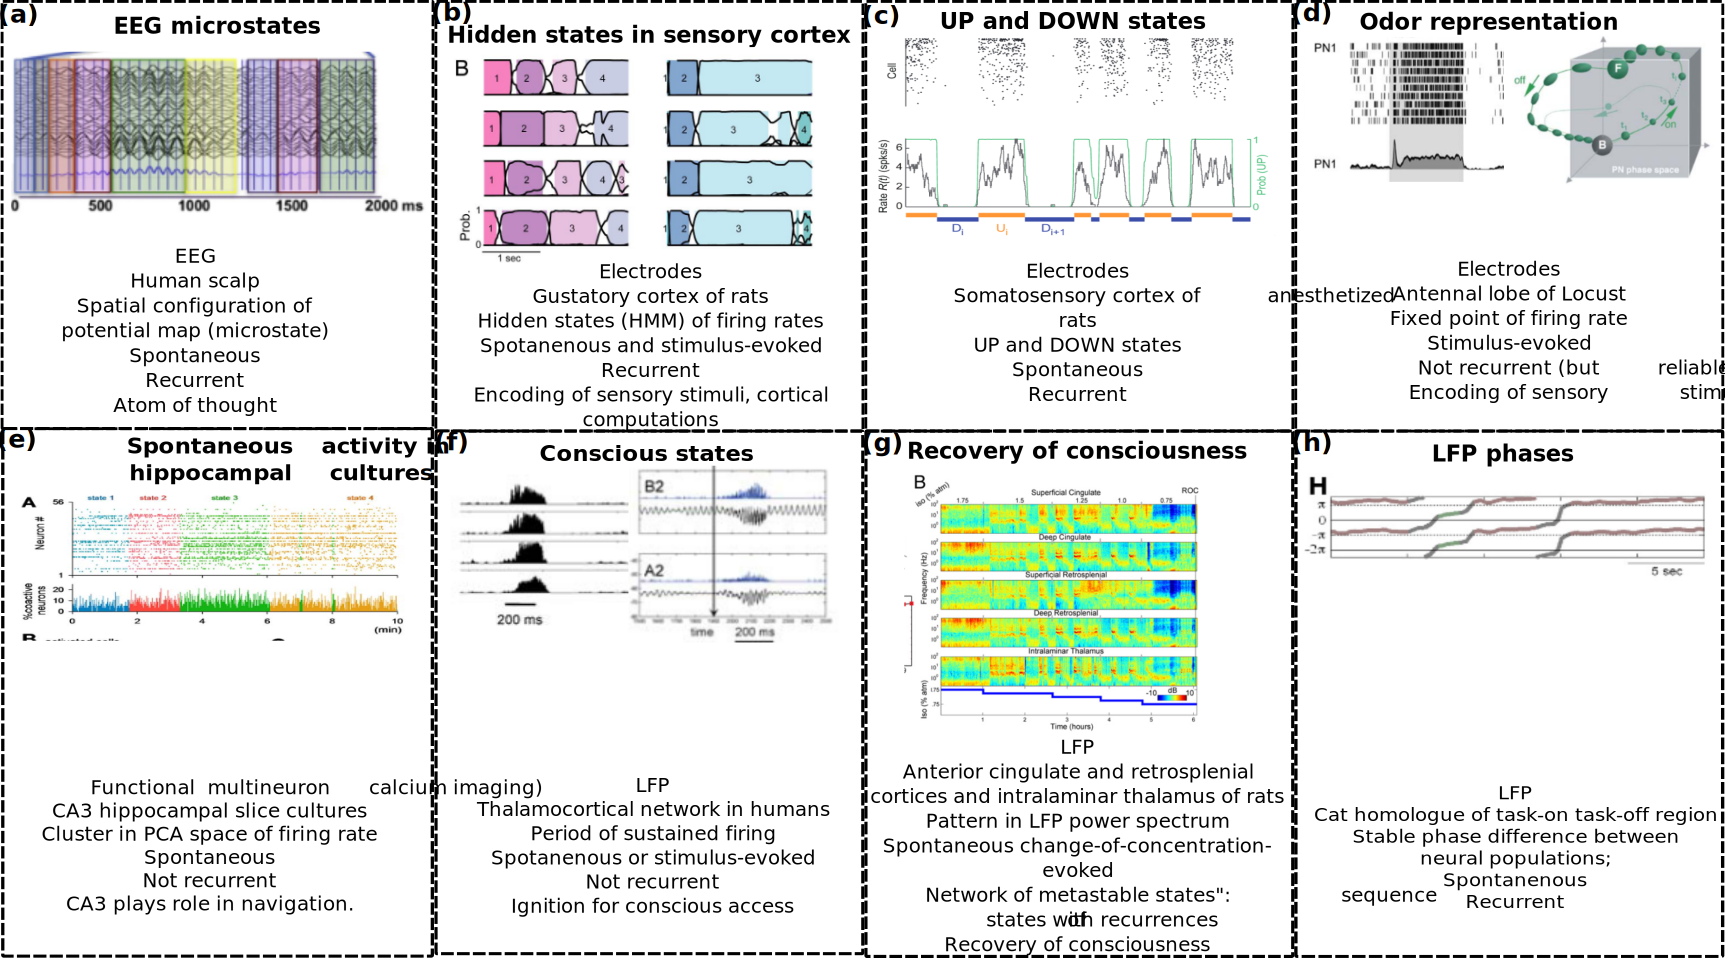
\includegraphics[width=\textwidth]{observationsmetastability.png}
    \caption{\textbf{Brain activity typically evolves as a sequence of well-defined states that are transient but long lived.} The panels illustrate important observations taken from the literature, namely EEG microstates \cite{michel2017eeg}, hidden Markov states of firing rates \cite{brinkman2022metastable}, UP and DOWN states \cite{jercog2017updown}, cortical wave patterns \cite{townsend2015emergence}, epileptic seizures \cite{wenzel2019acute}, and bursting in central pattern generators \cite{sakurai2016recruitment}. Each observation is explained in detail in the main text, and is classified into subtypes of metastability that we define in the Sec.~\ref{sec:subtypes}.}
    \label{fig:observationsmetastability}
\end{figure*}

As a first example, Fig. \ref{fig:observationsmetastability}A shows time-series of electroencephalography (EEG) measurements performed in resting humans with eyes closed (taken from \cite{michel2017eeg}). Colors indicate \Emph{EEG microstates}, identified from the spatial configuration of the electric potential amplitude of each electrode. These microstates remain almost stationary for roughly $\SI{100}{\milli\second}$ \cite{vandeville2010eeg, lehmann1987eeg}, and then give way to other microstates.

Figures \ref{fig:observationsmetastability}B-C show results based on firing rates of neurons. In particular, Fig. \ref{fig:observationsmetastability}B shows exemplary sequences of states adapted from Ref. \cite{brinkman2022metastable}. The states are characterized by roughly stationary behavior in the firing rates of neurons in the gustatory cortex of rats, and are identified via the technique of \Emph{hidden Markov models} (HMM). Each state lasts for roughly an order of magnitude longer than the transitions between any state \cite{jones2007natural, lacamera2019cortical, mazzucato2019expectation, recanatesi2021metastable, brinkman2022metastable}. This is observed during both spontaneous and stimulus-evoked activity, and the sequence of such states is shown to encode the stimuli presented to the animals \cite{lacamera2019cortical, mazzucato2019expectation}. These states are proposed to serve as a ``substrate for internal computations" in the brain \cite{lacamera2019cortical}. Similar results have also been reported in the frontal cortex of monkeys during a delayed localization task \cite{abeles1995cortical, seidemann1996simultaneously}.

Figure \ref{fig:observationsmetastability}C shows sequences of sustained firing (significant activity, \Emph{UP states}) and silence (\Emph{DOWN states}) in the firing rates of the deep layers of the somatosensory cortex of urethane-anesthetized rats (adapted from \cite{jercog2017updown}). Each state lasts for a significant time, with quick transitions between them \cite{jercog2017updown}. These states are ubiquitously observed in spontaneous activity \cite{luczak2007sequential, jercog2017updown}. 

Figure \ref{fig:observationsmetastability}D shows a sequence of complex \Emph{wave patterns} identified in the cerebral cortex of anesthetized marmoset monkeys, taken from Ref. \cite{townsend2015emergence} (Copyright 2015 Society for Neuroscience). Starting from local field potential data from multiple electrodes, they created a spatial map for the phases of the oscillations, filtered at the $\delta$ band ($1-\SI{4}{\hertz}$), from which they identified different spatiotemporal patterns, classified as plane waves (PW), synchrony (SY), node, from a source or sink (ND), spiral (SP), and saddle (SA) \cite{townsend2015emergence}. These patterns repeat across the time series, but the probabilities of switching from one pattern to another differs from pattern to pattern (i.e., there is preferential switching between patterns) \cite{townsend2015emergence}.
% The firing rate of neurons in slice cultures of the hippocampal CA3 region was found to evolve also as sequences of discrete, long-lasting states, separated by quick transitions \cite{sasaki2007metastability} (Fig. \ref{fig:observationsmetastability}D). The figure was taken from \cite{sasaki2007metastability} (Copyright 2007 Society for Neuroscience). Each state is identified by clustering algorithms applied to the space spanned by the principal components obtained from Principal Component Analysis (\Emph{PCA}) of the firing rates. The figure shows the raster plot of the firing, and the total activity, with colors denoting each state \cite{sasaki2007metastability}.

Mazor and Laurent \cite{mazor2005transient} (not included in the figure) measured the firing rate of neurons in the antennal lobe of locusts as the animals were presented with a variety of odor pulses. Their results suggest that, for long pulses (lasting more than $\SI{2}{\second}$), spiking activity in the antennal lobe switches between a baseline fixed point and an odor-specific fixed-point, which can last for a few seconds. Interestingly, the transition epochs between the two fixed points were found to contain the most amount of information about the stimuli, suggesting an important role for them in neural computations \cite{mazor2005transient, rabinovich2008transientdynamics}.

Figure \ref{fig:observationsmetastability}E shows the neural activity recorded by two-photon calcium imaging in mouse neocortex \cite{wenzel2019acute} (Copyright 2019 Society for Neuroscience). The population is being invaded by a propagating \Emph{epileptic seizure}, which appears in the middle of the time-series, and is characterized by sustained firing of a large number of neurons. Traveling as a wave, it transiently replaces the baseline state, in which firing is more sparse and distributed. In this study, a pharmacological agent was applied to a specific region of the cortex to induce the seizures.

% Figure \ref{fig:observationsmetastability}E shows that metastable states also occur in the context of consciousness. The global neuronal workspace theory of consciousness proposes that we become conscious of a certain object (e.g. a stimulus) when the representation of that object is broadcast from local processing regions into a variety of spatially distributed regions, which form the global workspace \cite{mashour2020conscious}. This global broadcast is known as \Emph{ignition}, and is achieved through the sustained firing of the involved areas; this is shown in panel E for the local-field potential (LFP) and spikes in area D2 of the model studied in \cite{dehaene2005ongoing}. The figure is adapted from \cite{dehaene2005ongoing}. The activity of workspace neurons is thus characterized by discrete episodes of spontaneous coherent activation, with sustained firing, and quick transitions between them \cite{michel2017eeg}.


Figure \ref{fig:observationsmetastability}F shows the swim motor pattern in intracellular recordings of two neurons that belong to the swim central pattern generator of the mollusk \textit{Tritonia} \cite{sakurai2016recruitment} (adapted from Ref. \cite{sakurai2016recruitment}). These neurons respond by \Emph{bursting} to stimulation in a nerve called PdN3. These bursts are phenomenologically similar to those shown later in Fig. \ref{fig:mechanismsmetastability}E (though their mechanisms might differ), and demonstrate the alternation between periods of sustained firing and periods of silence. Central pattern generators \cite{marder2001central} contain various examples of metastable states. 

Another work (not included in the figure) has also found that the power spectrum of local-field potential (LFP) recordings in rats progresses as a sequence of relatively stationary states lasting for some time before rapidly transitioning to other states \cite{hudson2014recovery} (see e.g. Fig. 2 of Ref. \cite{hudson2014recovery}). This was observed as the rats recovered consciousness, when the concentration of an anesthetic was progressively decreased. The authors argue that the existence of well-defined metastable states is crucial for the fast recovery of consciousness \cite{hudson2014recovery}.

Additionally, we remark that several other regimes could be mentioned in this section, such as other seizures \cite{curtis2015initiation, babloyantz1986low}; sleep spindles \cite{fernandez2020sleep}, transient patterns of circular waves that repeatedly travel across the cortex over sleep and may aid the consolidation of memories \cite{muller2016rotating}, and the phases of local-field potentials in cats at rest \cite{tognoli2014metastable, popa2009constracting}. Other results are also discussed in Ref. \cite{tsuda2009hypotheses}.

% We also note that some works mentioned previously may have not necessarily used the term metastability in their respective papers. \lm{Finally,} we note that some works interpret metastability differently than the idea of long-lasting states, and they were not included here.

\subsection{Current formulations}\label{sec:currentformulations}

Several theoretical formulations have been discussed as a result of the observations of metastability in the brain. However, despite their large applicability, such formulations often depend on the specific context of their observations. To illustrate this issue, we depict in Figs. \ref{fig:definitionsmetastability}A-F the main formulations of metastability that we have identified in the neuroscience literature.

We can generalize those from Figs.~\ref{fig:definitionsmetastability}A-E as considering metastability to be a regime with a type of variability in the dynamics. This variability can be directly observed in different \textit{patterns of activity} (Fig. \ref{fig:definitionsmetastability}A) \cite{friston1997transients, friston2000transients, varela2001brainweb, roberts2019metastable}, or \textit{patterns of synchronization} (Fig. \ref{fig:definitionsmetastability}B) \cite{cabral2011role, deco2017dynamics, deco2016metastability, poncealvarez2015restingstate, aguilera2016extended}. In some cases, abstract states can be identified through some technique, such as Hidden-Markov model \cite{mazzucato2015dynamics, lacamera2019cortical, brinkman2022metastable} or PCA analysis \cite{sasaki2007metastability}. Then, metastability is said to be the variability of these states (Fig. \ref{fig:definitionsmetastability}C) \cite{mazzucato2015dynamics, lacamera2019cortical, afraimovich2010longrange, alderson2020metastable, lee2017linking, vasa2015effects, hellyer2014control, naik2017metastability, rabinovich2008transientcognitive, cavanna2018dynamic, werner2007metastability, bhowmik2013metastability}. In other works, metastability is said to occur due to variability of trajectories along different \textit{regions of phase space} (which is, roughly, a space composed of the variables or observables of the system) (Fig. \ref{fig:definitionsmetastability}D) \cite{hudson2017metastability, graben2019metastable}, or along different positions in an \textit{energy landscape} (Fig. \ref{fig:definitionsmetastability}E) \cite{gili2018metastable, cavanna2018dynamic, aguilera2016extended, hudson2017metastability}. Another, more distinct, formulation of metastability is that of a regime \textit{integration-segregation}, in which neural assemblies transiently synchronize and desynchronize (Fig. \ref{fig:definitionsmetastability}F) \cite{deco2015rethinking, fingelkurts2001operational, tognoli2014metastable, tognoli2014enlarging, bressler2016coordination, kelso2012multistability, hellyer2015cognitive}. 

Furthermore, we remark that, while some works explicitly mention a time-scale separation in metastability \cite{hudson2017metastability, brinkman2022metastable}, others do not. The latter can be problematic, as it implies that even states with arbitrarily short durations can be regarded as metastable.
Works also differ in regards to the possible mechanisms giving rise to metastability. Some consider that the variability in the dynamics needs to be spontaneous, occurring in autonomous systems (Fig. \ref{fig:definitionsmetastability}G) \cite{sasaki2007metastability, kelso2012multistability, roberts2019metastable, fingelkurts2008brainmind, cavanna2018dynamic}, while others argue that the variability must be externally induced, occurring in non-autonomous systems (Fig. \ref{fig:definitionsmetastability}G\supprime) \cite{jercog2017updown, hudson2017metastability}. A combination of both is also found in Refs. \cite{brinkman2022metastable, friston2000transients, lacamera2019cortical}.  
Finally, another source of differences is in the repeatability of metastable regimes: some works consider metastable states as repeatable  (Fig. \ref{fig:definitionsmetastability}H) \cite{graben2019metastable}, while others consider them as non-repeatable (Fig \ref{fig:definitionsmetastability}H\supprime). Examples of these types of metastability are shown in the observations in Fig. \ref{fig:observationsmetastability}.
%
\begin{figure*}[htb]
    \centering
    \includegraphics[width=\textwidth]{definitionsmetastability.png}
    \caption{\textbf{Formulations of metastability in the neuroscience literature.} A common theme among these is the presence of transitions between certain aspects of the system's dynamics (e.g., between activity patterns). The upper part of the figure illustrates what these aspects are in each definition, and the bottom part shows characteristics of the transitions. Further details are available in the main text.}
    \label{fig:definitionsmetastability}
\end{figure*}

\section{A unifying framework of metastability}\label{sec:framework}

Here, we propose to unify the observations and formulations of metastability into a single framework. We start with a general, context-independent, definition of metastability that acts as an umbrella term including the other formulations as distinct subtypes. This definition already facilitates meaningful comparisons between the various observations of metastability. Then, using insights from nonlinear dynamical systems theory, we expand the framework by providing a variety of mechanisms leading to metastability. 

\subsection{A general definition}
\label{sec:definitions}
A unified framework for metastability relies on a general definition of the behavior, which itself relies on the notion of metastable states. To this end, we first establish the concept of a state as an \textbf{epoch of the dynamics with typical and unique properties}. The dynamics are specified, both experimentally and theoretically, by observables (e.g., local-field potential in EEG, or neuronal firing rates). Properties can then be identified from these observables, such as wave patterns, hidden Markov states, or synchronization patterns, and they are often stationary or quasistationary in the statistical sense for the state's duration \cite{michel2017eeg, brinkman2022metastable, mazor2005transient} (as discussed in Sec. \ref{sec:observations}). 

With these concepts, we propose that \Emph{states are metastable if they are transient but long-lived}. Thus, a metastable state is expressed continuously for a long time, but is eventually left by the system. More quantitatively, we define a state's duration $\tau$ as finite but longer than some characteristic time $\tau_0$ defining its dynamics, such that $\tau_0 < \tau < \infty$.
% The first definition we propose is easy: metastability occurs when a system has metastable states. Then, we define (again) a \Emph{state as an epoch of the dynamics with typical and unique properties}. These properties are features (i.e. quantifiers, or observables) of the dynamics that characterize the state and are stationary or quasistationary in time in the statistical sense (i.e. their statistics remain roughly constant throughout the state). As we have seen in Fig. \ref{fig:observationsmetastability}, a state can be a pattern of activity (such as a wave pattern), of firing rates (such as a hidden Markov state), of synchronization, among many other possibilities. Then, we propose that \Emph{states are metastable if they are transient but long-lived.} A metastable state is expressed continuously for a long time, but is eventually left. More quantitatively, we can say a state is metastable if its duration $\tau$ is finite but longer than some characteristic time $\tau_0$ defining it (i.e. $\tau_0 < \tau < \infty$).

Our definition of metastability is based solely on observables of a system. An important advantage of this approach is its ability to quickly identify metastability from experimental neurobiological data. Besides its experimental accessibility, the definition also connects directly to theoretical concepts of nonlinear dynamical systems theory, which allows for a theoretical framework based on the experimental observations that can also lead to deep theoretical insights. But to establish this connection, we first need to explore the concept of phase space: the phase space of a system is a multidimensional space in which each dimension corresponds to an observable that describes the system. For example, consider a system of $N$ neurons whose observables are their firing rates. The instantaneous firing rates at each time correspond to a point in this $N$-dimensional phase space. An equilibrium, in which the system's state is constant in time (e.g., constant firing rates across time), is a single point in this space, while a continuous periodic solution is a closed loop. The theory of dynamical systems shows that the geometry of structures like these underlies the systems' dynamics: the time evolution of a system is represented by trajectories in this phase space, and the stability of structures there can be interpreted according to geometrical properties in this space. In particular, an equilibrium  solution is stable if it attracts trajectories from all directions, and unstable if it repels trajectories from at least one direction. This notion allows us to extract a clear and simple \textit{dynamical principle} that underlies systems with metastability: metastable states occur due the coexistence of attracting and repelling directions around that state in phase space (as proposed similarly in Refs. \cite{tognoli2014metastable} and \cite{kaneko2003chaotic}). The ability of metastable states to retain trajectories is thus due to their attracting directions, and their finite duration is due to their repelling directions that push the trajectories away. 

Furthermore, the phase space view also allows us to better specify the characteristic time $\tau_0$ through the tools from dynamical systems theory \cite{lai2009transient}. For continuous-time systems without external perturbations, $\tau_0$ can be, for instance, (i) the period of periodic oscillations, (ii) an average period for chaotic oscillations, or (iii) a characteristic return time to equilibria (fixed points, when perturbed) that can be obtained from the eigenvalues of the Jacobian at those points \cite{strogatz2002nonlinear}. For systems with external perturbations (driven systems), $\tau_0$ can be the period or a characteristic time of the forcing. In noisy systems, described by stochastic differential equations, metastable behaviors have an explicit timescale separation, and their characteristic times can be obtained from the eigenvalues of transfer operators \cite{bittracher2018transition, bittracher2021dimensionality}. Finally, for discrete-time systems, $\tau_0$ can be simply one iterate (i.e., the time-step) \cite{lai2009transient}. %In the next section, we explore and illustrate these geometrical ideas in more detail.


\subsection{Dynamical mechanisms for metastability}
\label{sec:mechanisms}
Following our general definition of metastability, we now explain some important mechanisms that can generate metastability, all of which are known from nonlinear dynamical systems theory, but only a few of which have been discussed previously in the literature \cite{graben2019metastable, cavanna2018dynamic}. 

We start with the role of \Emph{noise in a multistable system}. Specifically, we consider the simplest case, in which a particle moves with friction under the influence of an energy landscape composed of two wells separated by a hill. Without any external perturbation, the particle's trajectory converges to the bottom of one of the two wells, depending on its initial condition (where it is released and with which velocity). The bottom of each well therefore corresponds to a long-term state, called a \textit{fixed-point attractor}. Since the system has two attractors, it is called bistable. 
When a periodic forcing is added to the system, the particle's trajectories evolve periodically around the well, on a \textit{periodic attractor}. Adding noise on top of this enables the trajectories to occasionally cross the hill separating the two wells. The trajectories thus spend time around one well, then hop to the other well, and repeat this cycle indefinitely. This phenomenon is called \textit{attractor hopping} \cite{kraut2002multistability}, and is shown in the time-series of the particle's position in Fig. \ref{fig:mechanismsmetastability}A. The system is no longer bistable, but it does have two metastable states, each corresponding to the dynamics around one well. This can also be seen in the particle's phase space, spanned by its position $x$ and velocity $dx/dt$, shown in Fig. \ref{fig:mechanismsmetastability}A\supprime. The times spent on each metastable state (called residence times, dwell times, or also permanence times) follow a probability distribution, such as an exponential distribution for Gaussian white noise \cite{hanggi1986escape} (Figure \ref{fig:mechanismsmetastability}A\textsuperscript{\everymodeprime\everymodeprime}). This mechanism of noise-induced transitions in multistable systems has been proposed for several observations of metastability in the brain \cite{brinkman2022metastable, hudson2017metastability}.

Metastable states can also occur in the absence of noise or any external input, due different deterministic mechanisms. We concentrate now on some of these, starting with a \Emph{stable heteroclinic cycle}, which occurs here on a firing-rate model derived from three synaptically-coupled Hodgkin-Huxley neurons \cite{ashwin2011criteria}. Figure \ref{fig:mechanismsmetastability}B shows a trajectory on such a cycle, performing a sequential alternation between three distinct states. Each state is a fixed point of saddle type, meaning it has specific attracting directions (stable manifold) and repelling directions (unstable manifold) in phase space. Because of this, trajectories approach each saddle point along its stable manifold - and potentially spend a long time near it - but eventually depart along its unstable manifold. This makes each saddle point a metastable state. But the heteroclinic cycle itself is stable, since the manifolds are connected in such a way that trajectories repelled from one saddle point are attracted to the next, and so the trajectories cycle through each saddle sequentially in the same order eternally. Figure \ref{fig:mechanismsmetastability}B shows the time evolution of one variable, with each color representing one state, and Fig. \ref{fig:mechanismsmetastability}B\supprime shows the state space with the saddles and a trajectory. Each time a trajectory approaches a saddle, it comes ever closer to it, and so spends ever more time near it, leading to the sequence of residence times shown in panel B\ssupprime. Importantly, it can be shown that such heteroclinic cycles can globally attract trajectories \cite{nowotny2007dynamical} and are also conserved under small parameter changes (they are structurally stable) \cite{rabinovich2008transientcognitive}. 
Moreover, it has been shown in neural networks that heteroclinic cycles depend on the inputs to the neurons, such that the cycle is sensitive to the stimulus to the network \cite{rabinovich2001dynamical}. Once the stimulus is applied, and the cycle is defined, it is robust against noise. So this mechanism allows for robustness to noise while keeping sensitivity to inputs \cite{rabinovich2001dynamical, rabinovich2008transientcognitive}. The heteroclinic cycle also generates sequential ordering of patterns, which may be relevant for reliable neural computations \cite{fonollosa2015learning}. It has also been proposed as the mechanism behind experimental observations \cite{rabinovich2008transientcognitive, rabinovich2008transientdynamics, rabinovich2012information} and theoretically hypothesized as a mechanism for cognition \cite{fonollosa2015learning, rabinovich2014chunking}.
%
\begin{figure*}[hbt]
    \centering
    % \includegraphics[width=\textwidth]{mechanismsmetastability.pdf}
    \includegraphics[width=\textwidth]{mechanismsmetastability.png}
    \caption{\textbf{Dynamical mechanisms of metastability.} Each column corresponds to one mechanism, with the panels respectively showing a representative time-series, trajectories in phase space, and the distribution of residence times in each identified metastable state. Further details in the main text and Supplemental Material.}
    \label{fig:mechanismsmetastability}
\end{figure*}
% state is not necessarily the same as a single point in phase space - it can include more points.

Now we move to another example, which involves a \textit{chaotic attractor}. Unlike the fixed point and periodic attractors discussed so far, the trajectories on a chaotic attractor are fundamentally unpredictable, which occurs because nearby trajectories on the attractor diverge exponentially from each other in time. For the example, the chaotic attractor results from the merging of two previously separated attractors, both also chaotic. In this case, the merged chaotic attractor has two distinct subregions, each one corresponding to one of the attractors before the merging. These subregions trap trajectories for a considerable time, following an exponential probability distribution \cite{grebogi1983crises} (Fig. \ref{fig:mechanismsmetastability}C\ssupprime). So that both subregions are metastable states. Figures \ref{fig:mechanismsmetastability}C and C\supprime show the intermittency between each metastable state, colored either green or purple. This mechanism is called an \textbf{attractor-merging crisis}. 
It is interesting to note that the trajectories for this mechanism look similar to those for the noisy bistable systems (compare Figs. \ref{fig:mechanismsmetastability}A and \ref{fig:mechanismsmetastability}C). The key difference is that the transitions in the former are caused by noise, and in the latter they are caused by the deterministic dynamics of the system on the attractor, namely by a saddle periodic orbit mediating the crisis. Still, this highlights the often apparent similarity between noisy and chaotic dynamics, and the need for deeper analysis to distinguish between both \cite{boaretto2021discriminating}.

Similar dynamics occur as a result of an \textbf{interior crisis}, another mechanism. In it, a parameter change makes a chaotic attractor suddenly occupy a larger region of phase space, which can be roughly decomposed into an inner core, that the previous attractor occupied, and an outer core, where the expansion took place. Trajectories near this attractor intermittently switch between the inner and outer cores, with an exponential distribution of residence times. The attractors near both crises, attractor-merging and interior, are two of many concrete instances of an idea proposed by Friston \cite{friston2000transients}, who argues that different metastable states can live in different subregions of the same attractor. This idea is also valid for other mechanisms we discuss in the sequence.

In the two previous examples, the metastable states involved fixed points, periodic and chaotic attractors, all of which are said to be invariant - meaning that points belonging to these structures evolve to other points also belonging to them. Figure \ref{fig:mechanismsmetastability}D now shows that a metastable state can also correspond to a region of phase space without an existing invariant structure. This is the case near a saddle-node bifurcation of periodic orbits, leading to \Emph{type-I intermittency}. In time-discrete systems, it occurs when a pair of fixed points, a saddle (with attracting and repelling directions) and a node (only attracting directions) merge in phase space. The bifurcation destroys the saddle and the node, leaving behind only a \textit{ghost} of the node \cite{pomeau1979intermittency, pomeau1980intermittent, strogatz2002nonlinear}. In time-continuous systems, this mechanism occurs analogously for unstable and stable periodic orbits  \cite{medeiros2016trapping}, an example of which is the Lorenz system that we show in Fig. \ref{fig:mechanismsmetastability}D. Contrary to the stable limit cycle (or the node), the ghost is not invariant: trajectories on the ghost eventually exit it. Indeed, after the bifurcation, the trajectories converge to another attractor, such as a chaotic attractor for the system in the figure, where they have chaotic, irregular dynamics (purple part of Fig. \ref{fig:mechanismsmetastability}D). When they pass near the ghost, however, they spend a long time near it and become nearly periodic (green parts). Commonly, the ghost is embedded in the attractor of the system, as in this example, such that the trajectories get constantly reinjected near it after exiting, generating an asymptotic regime alternating between two metastable states: the ghost and the rest of the chaotic attractor \cite{pomeau1980intermittent}. The time spent on the ghost can be considerably long, but is finite for any fixed parameter \cite{pomeau1980intermittent}.
Chaos is a mechanism for re-injection in deterministic systems, but re-injection can also occur in systems with noise \cite{medeiros2016trapping}. 
This mechanism has been proposed by Kelso and colleagues as the mechanism for metastability in the brain \cite{kelso1991an, tognoli2014metastable}. It is another example of the general proposal by Friston \cite{friston2000transients}, since the trajectories here live on a chaotic attractor, which can nevertheless be separated in two distinct dynamical regimes: nearly-periodic (green) and chaotic dynamics (purple). 

Another mechanism that leads to metastable states is due to a \Emph{chaotic saddle}. A chaotic saddle is similar to a chaotic attractor, with the distinction that it also has repelling directions (it is thus the analogue of a saddle fixed point for a chaotic set) \cite{lai2009transient}. As a consequence, trajectories can stay near the chaotic saddle for potentially very long times, displaying chaotic dynamics, before eventually being expelled from it \cite{yorke1979metastable}. This is the purple structure in Figs. \ref{fig:mechanismsmetastability}E and E\supprime. This behavior characterizes the chaotic saddle as a metastable state. The residence times for different initial conditions near the chaotic saddle follow an exponential distribution \cite{grebogi1983crises} (Fig. \ref{fig:mechanismsmetastability}E\ssupprime). We remark that trajectories on the chaotic saddle resemble the ignition behavior leading to conscious access shown in Ref. \cite{dehaene2005ongoing}.
A chaotic saddle has been reported in networks of spiking neurons \cite{ansmann2016selfinduced}, in which, interestingly, it can be subdivided into three distinct dynamical regimes, corresponding to three subregions, which are all intermittently accessed. Therefore, also every subregion of that chaotic saddle can be considered metastable. Chaotic saddles have also been observed in other networks of spiking neurons \cite{keplinger2014transient, lafranceschina2015impact, hartle2017transient, kaminker2019alternating}.

There are several other dynamical mechanisms for metastability beyond the ones discussed previously. One example is \Emph{on-off intermittency}, which is common, for instance in systems that can completely synchronize \cite{ashwin1994bubbling, ott1994blowout, saha2017extreme}, and occurs during transitions from synchronization to desynchronization induced by changing the global coupling strength. During these transitions, systems with on-off intermittency have trajectories that intermittently switch from a synchronized regime to a desynchronized one and back. The mechanism for this intermittency, and its statistical scaling, has been studied in detail \cite{ platt1993onoff, heagy1994characterization, hammer1994experimental, cenis1997symmetry}. It is one out of many possible mechanisms that can realize the coexistence of integration (synchronization) and segregation (desynchronization), often mentioned as a crucial need for the brain \cite{fingelkurts2001operational, tognoli2014metastable, tognoli2014enlarging, deco2015rethinking}. It is also a possible mechanism for the intermittent switching between UP and DOWN states exemplified in Fig. \ref{fig:observationsmetastability}C. Furthermore, evidence for on-off intermittency has been reported for EEG data of non-convulsive paroxysmal (high-amplitude) activity in rats with genetic absence epilepsy \cite{hramov2006onoff}. The study identified a power-law distribution of residence times characteristic of on-off intermittency in regular brain activity, which alternated with the epileptic paroxysms.
A very similar mechanism is in-out intermittency \cite{ashwin1999transverse, ashwin2001influence,saha2018characteristics}. In addition, evidence for yet another type of intermittency, known as type-III intermittency \cite{pomeau1979intermittency}, has been reported in \cite{velazquez1999type}.

Another example of metastability is \Emph{bursting} behavior, characterized by quick firing of spikes followed by a quiescent period (as in Fig. \ref{fig:observationsmetastability}F). Bursting is a ubiquitous mode of firing in neurons \cite{fox2015bursting}, and can have important functional roles due to its ability to generate more robust responses \cite{swadlow2001impact}. A simple model displaying bursting is the Hindmarsh-Rose neuron \cite{hindmarshmodel1984}. In it, an adaptation current causes the switching between the tonic spiking and the silence \cite{hindmarshmodel1984}. The whole trajectory is on stable limit cycle, but can still be decomposed into the tonic spiking and the silence, each of which can be considered metastable. This is yet another example of the idea proposed by Friston in \cite{friston2000transients}. 

A similar important behavior is \Emph{mixed-mode oscillations}, in which trajectories alternate between periods of small amplitude (e.g., sub-threshold) and large amplitude oscillations (e.g., spikes) \cite{rotstein2014mixedmode}. There are various mechanisms for mixed-mode oscillations, which can involve either forcing the system to induce changes of parameters or through an adaptation variable that enables the switching between the two modes \cite{desroches2012mixed, rotstein2014mixedmode}.

Another important example of metastable behavior is \Emph{chaotic itinerancy} \cite{kaneko2003chaotic}. This phenomenon has also been discussed in the context of neuroscience \cite{freeman2003evidence, tsuda2009hypotheses, tsuda2015chaotic}, and includes several specific mechanisms, and thus is also an umbrella term, but more specific than metastability as we define it here.


\subsection{Subtypes of metastability}
\label{sec:subtypes}
The definition of metastability that we propose leads naturally to the classification of several subtypes. For instance, spontaneous and driven metastability (illustrated in Figs. \ref{fig:definitionsmetastability}G-G\supprime respectively). In spontaneous metastability, the transitions between states occur spontaneously, without the need for external perturbations to the system. In this case, the system may still be open (i.e., subject to external perturbations, such as noise), but the mechanism for the transitions is intrinsic to the system and can be separated from the perturbations. Conversely, in driven metastability the transitions occur due to factors external to the system itself, such as the presentation of a stimulus. Another important pair of subtypes is repeatable metastability and non-repeatable metastability (Figs. \ref{fig:definitionsmetastability}H-H\supprime). These are characterized by whether the metastable states eventually repeat in the time series or not. To avoid confusion, we emphasize that the repeated object is the metastable state (for instance, the neighborhood of some saddle periodic orbit), and not a single point in that space (which can only be visited repeatedly in periodic orbits). The case of non-repeatable states is sometimes called metastability en route to ground state \cite{brinkman2022metastable}. Note that the observations in Figure \ref{fig:observationsmetastability} are already classified into these subtypes. 

Each mechanism has distinct but important functional roles: spontaneous metastability enables transitions between states without the expenditure of additional energy to stimulate the transitions \cite{tognoli2014metastable}, and guarantees that a system does not get stuck in the same state \cite{ito2008dynamics}; driven metastability is important for direct control of the transitions, and in stimulus-evoked cases.

The mechanisms we have shown in Sec. \ref{sec:mechanisms} illustrate these different subtypes. There, only the first requires noise for the transitions; the rest have spontaneous transitions that can be robust with respect to noise. Furthermore, there the chaotic saddle (Fig. \ref{fig:mechanismsmetastability}E) is not repeatable, as it occurs only once in the observation, though the residence may be extremely long; the other metastable states shown are repeatable. Another distinction that can be made is in regards to the distribution of residence times. As shown in the third panel of each mechanism in Fig. \ref{fig:mechanismsmetastability}, the behavior of the residence times differs across some mechanisms: they may be extremely long (noisy bistable, especially for weak noise, heteroclinic cycle, attractor-merging crisis, and chaotic saddle); they may have a maximum value (saddle-node bifurcation), or even a constant value (for the periodic bursting in Hindmarsh-Rose neurons \cite{hindmarshmodel1984}, not shown in the figure).

\section{Conclusions and outlook}

Throughout this paper, we argue that the observations and formulations of metastability in neuroscience have so far been mostly restricted to each study's specific context. Our aim is to take these context-specific ideas and unify them into a general, context-independent, framework that can be used to both describe and understand metastable brain dynamics. We start by proposing a general definition of metastability as a regime with transient states that last for a significant amount of time. Metastability then becomes an umbrella term encompassing phenomena characterized by transient but long-lived states, and each context-dependent case then fits neatly into a subtype of metastability.  The definition depends solely on observable aspects of the system, making it directly applicable to experimental data. 

On top of this dynamical aspect, the definition of metastability can be connected to the theory of nonlinear dynamical systems, allowing us to extract a simple dynamical principle underlying metastable states: the coexistence of attracting and repelling directions in phase space.  This general principle can occur due to several dynamical mechanisms. Using again the theory of nonlinear dynamical systems, we discuss some of these mechanisms, providing further insights into previously discussed mechanisms and proposing several additional ones. This approach provides insights on the distinct subtypes of metastability, for instance on the difference between noise-induced and spontaneous transitions between metastable states. It also gives further insights into mechanisms already proposed in the literature. One example is the several concrete instances we have provided for an abstract mechanism proposed by Friston in \cite{friston2000transients} of metastable states corresponding to sub-regions of a same attractor. Another example is the proposal of additional mechanisms that can account for the coexistence of segregation and integration, which go beyond what was already proposed in the literature. 

Future works can use this framework to further develop the current understanding of metastable brain dynamics, since each dynamical mechanism has distinctive signatures that can be explored to identify them from experimental data. Knowledge of the mechanisms is crucial for developing better control of the systems and for better predicting their behavior. This possibility constitutes an exciting avenue of future research, that requires both theoretical works exploring the signatures of each mechanism and experimental works in obtaining and dealing with data to find those signatures. Recent advancements in the identification of system equations from data \cite{voss2004nonlinear, brunton2016discovering, tabar2019analysis, anvari2016disentangling} could prove very fruitful here. Therefore, we believe that the framework we establish here is crucial in uniting the observations and formulations of metastability in neuroscience, and also in uniting several research areas towards the goal of understanding metastable brain dynamics. 


\section*{Acknowledgments}
We would like to thank inspiring discussions with James A. Yorke, Klaus Lehnertz, and Nicolás Rubido. K.L.R. was supported by the German Academic Exchange Service (DAAD). E.S.M acknowledges the support by the Deutsche Forschungsgemeinschaft (DFG) via the project number 454054251. B.R.R.B. acknowledges the support of the São Paulo Research Foundation (FAPESP), Brazil, Proc. 2018/03211-6 and 2021/09839-0. This work was partially supported by BrainsCAN at Western University through the Canada First Research Excellence Fund (CFREF), the NSF through a NeuroNex award (\#2015276), the Natural Sciences and Engineering Research Council of Canada (NSERC) grant R0370A01, and the Western Academy for Advanced Research. R.C.B gratefully acknowledges the Western Institute for Neuroscience Clinical Research Postdoctoral Fellowship.

\section*{Supplementary material}
\subsection{Models}
The code used to generate Figure 3 in the main text is available in the GitHub repository \cite{rossi2022repository}. All the code is done in the Julia computational language \cite{bezanson2017julia}; integration was done with the package DifferentialEquations.jl \cite{rackauckas2016differential}, with the aid of packages DynamicalSystems.jl \cite{datseris2018dynamical} and DrWatson.jl \cite{datseris2020drwatson}. Plots were made with Makie.jl \cite{danisch2021makie}.

\subsubsection{Noisy bistable}
The noisy bistable system, also known as the noisy Duffing oscillator \cite{strogatz2002nonlinear}, is given by:
\begin{align}
    \dot{x} &= v + \eta_1 \dot{W}\\ 
    \dot{v} &= -ax^3 + bx -c -dv + f\cos(\omega t) + \eta_2 \dot{W},
\end{align}
with $\dot{W}$ describing a white Gaussian noise. The equations describe the evolution of a particle on a double-well (quartic) potential $U(x) = ax^4/4 -bx^2/2 +cx$ being periodically driven and with noise.
The parameters used were $a=0.5$; $b=8.0$, $c=0.0$, $d = 0.2$, $f = 0.0$, $\omega = 1.0$, $\eta_1= \eta_2 = 0.18$, with initial condition $(0, 0)$. 

% Each well corresponds to a fixed point in this system. Without noise, trajectories would converge to one of the fixed points and stay there indefinitely, as they would be stable. But the noise kicks trajectories away from the fixed points, such that, the fixed point now become metastable. For noise amplitudes that are not too high, the trajectory keeps alternating between dwelling near one (now metastable) fixed point and dwelling near the other, as shown in Fig. \ref{fig:observationsmetastability}(a). 

\subsubsection{The heteroclinic cycle}
The heteroclinic cycle occurs in a rate model derived from Hodgkin-Huxley type neurons with synaptic coupling \cite{ashwin2011criteria}. The equations are given by:
\begin{align}
\tau\dot{s_i} &= \left( r_i - s_i/2 \right) \frac{S_\mathrm{max} - s_i}{S_\mathrm{max}} \\
\tau\dot{r_i} &= x_0 F\left( I - \sum_{j=1}^N g_{ij} s_j \right) \tau - r_i \\
\end{align}
for $i = 1, 2, 3$, with 
\begin{equation}
    F(x) = \exp(-\epsilon/x) [\max(0, x)^\alpha ]. 
\end{equation}

The matrix $g$ is constructed such that $g_{21} = g_{32} = g_{13} = g_1$, $g_{12} = g_{23} = g_{31} = g_2$ and $g_{11} = g_{22} = g_{33} = 0$. The parameters are $\tau = 50$, $\epsilon = 10^{-3}$, $I = 0.145$, $S_\mathrm{max} = 0.045$, $g_1 = 3.0$, $g_2 = 0.7$, $x_0 = 2.57 \times 10^{-3}$, and $\alpha = 0.564$.

The numerical integration is best done with a change of coordinates $z_i \equiv \log(S_\mathrm{max} - s_i)$, which reduces the numerical precision difficulties associated with the trajectory getting too close to the stable manifold of the fixed points. The initial condition was $(0.5, 0.2, 0.4, 0.9, 0.5, 0.6)$. 

% The heteroclinic cycle as a whole is an attractor of the system. But the trajectories on the cycle alternate between the three saddle fixed points. Each saddle has distinct properties (their position in phase space), and the duration near them is long, so each saddle is a metastable state.

\subsubsection{Attractor-merging crisis}
We have provided an example of attractor-merging crisis for the Duffing oscillator, whose dynamics is described by \cite{ishii1986breakdown}: 
%
\begin{align}
    \dot{x} &= v \\ 
    \dot{v} &= -ax^3 + bx -dv + f \cos(\omega t) 
\end{align}

with parameters $a = 100$, $b = 10$, $d = 1.0$, $f = 0.852$, $\omega = 3.5$ and initial condition $(x,v) = (0.11, 0.11)$.

\subsubsection{Type I intermittency}
The system used to obtain the type I intermittency is the Lorenz63 model \cite{lorenz1963deterministic}. The equations are given by 
\begin{align}
    \dot{x} &= \sigma(y - x) \\ 
    \dot{y} &= x(\rho - z) - y \\ 
    \dot{z} &= xz - \beta z \\
\end{align}

The parameters used in the figure are $\sigma = 10$, $\beta = 8/3$ and $\rho = 166.1$, based on \cite{yorke1979metastable}. The parameter used to obtain a stable limit cycle (before the saddle-node bifurcation) was $\rho = 166.06$. The initial condition was $(0.1, 0.1, 0.1)$. 


% The trajectories alternate between the ghost of the limit cycle (where they have almost periodic behavior) and between chaotic behavior. In the example shown in Fig. \ref{fig:observationsmetastability}(c), the periodic regime lasts for a long time, compared to its own period, so it is a metastable state. The chaotic regime cannot be considered metastable in the figure, since its duration is too short. For other parameter choices, the chaotic phase can be much longer, and then it would be characterized as metastable. 

\subsubsection{Chaotic saddle}
The chaotic saddle shown in the figure occurs in the Ikeda system \cite{alligood1997book}, which has discretized time:
\begin{align}
    x_{n+1} &= a+b(x_n \cos(t_n) - y \sin(t_n)) \\ 
    y_{n+1} &= b(x_n \sin(t_n) - y_n \cos(t_n)), \\ 
\end{align}
with 
\begin{equation}
    t_n = c - \frac{d}{1 + x^2 + y^2}.
\end{equation}
The parameters used for the chaotic saddle were $b = 0.9$, $c = 0.4$, $d = 6.0$, $a = 1.003$. The saddle occurs due to a boundary crisis, which occurs for a slightly smaller $a$. For reference, the value of $a$ used to obtain a chaotic attractor was $a = 0.997$. The initial condition was $(2.97, 4.15)$. This is the only mechanism in the figure where the initial condition is important: to reproduce the behavior, the trajectories need to be initialized near the chaotic saddle.



\begin{thebibliography}{123}%
\makeatletter
\providecommand \@ifxundefined [1]{%
 \@ifx{#1\undefined}
}%
\providecommand \@ifnum [1]{%
 \ifnum #1\expandafter \@firstoftwo
 \else \expandafter \@secondoftwo
 \fi
}%
\providecommand \@ifx [1]{%
 \ifx #1\expandafter \@firstoftwo
 \else \expandafter \@secondoftwo
 \fi
}%
\providecommand \natexlab [1]{#1}%
\providecommand \enquote  [1]{``#1''}%
\providecommand \bibnamefont  [1]{#1}%
\providecommand \bibfnamefont [1]{#1}%
\providecommand \citenamefont [1]{#1}%
\providecommand \href@noop [0]{\@secondoftwo}%
\providecommand \href [0]{\begingroup \@sanitize@url \@href}%
\providecommand \@href[1]{\@@startlink{#1}\@@href}%
\providecommand \@@href[1]{\endgroup#1\@@endlink}%
\providecommand \@sanitize@url [0]{\catcode `\\12\catcode `\$12\catcode
  `\&12\catcode `\#12\catcode `\^12\catcode `\_12\catcode `\%12\relax}%
\providecommand \@@startlink[1]{}%
\providecommand \@@endlink[0]{}%
\providecommand \url  [0]{\begingroup\@sanitize@url \@url }%
\providecommand \@url [1]{\endgroup\@href {#1}{\urlprefix }}%
\providecommand \urlprefix  [0]{URL }%
\providecommand \Eprint [0]{\href }%
\providecommand \doibase [0]{https://doi.org/}%
\providecommand \selectlanguage [0]{\@gobble}%
\providecommand \bibinfo  [0]{\@secondoftwo}%
\providecommand \bibfield  [0]{\@secondoftwo}%
\providecommand \translation [1]{[#1]}%
\providecommand \BibitemOpen [0]{}%
\providecommand \bibitemStop [0]{}%
\providecommand \bibitemNoStop [0]{.\EOS\space}%
\providecommand \EOS [0]{\spacefactor3000\relax}%
\providecommand \BibitemShut  [1]{\csname bibitem#1\endcsname}%
\let\auto@bib@innerbib\@empty
%</preamble>
\bibitem [{\citenamefont {Contreras}\ \emph {et~al.}(1996)\citenamefont
  {Contreras}, \citenamefont {Destexhe}, \citenamefont {Sejnowski},\ and\
  \citenamefont {Steriade}}]{contreras1996control}%
  \BibitemOpen
  \bibfield  {author} {\bibinfo {author} {\bibfnamefont {D.}~\bibnamefont
  {Contreras}}, \bibinfo {author} {\bibfnamefont {A.}~\bibnamefont {Destexhe}},
  \bibinfo {author} {\bibfnamefont {T.~J.}\ \bibnamefont {Sejnowski}},\ and\
  \bibinfo {author} {\bibfnamefont {M.}~\bibnamefont {Steriade}},\ }\href
  {https://doi.org/10.1126/science.274.5288.771} {\bibfield  {journal}
  {\bibinfo  {journal} {Science}\ }\textbf {\bibinfo {volume} {274}},\ \bibinfo
  {pages} {771} (\bibinfo {year} {1996})}\BibitemShut {NoStop}%
\bibitem [{\citenamefont {Steriade}\ \emph {et~al.}(1993)\citenamefont
  {Steriade}, \citenamefont {McCormick},\ and\ \citenamefont
  {Sejnowski}}]{steriade1993thalamocortical}%
  \BibitemOpen
  \bibfield  {author} {\bibinfo {author} {\bibfnamefont {M.}~\bibnamefont
  {Steriade}}, \bibinfo {author} {\bibfnamefont {D.~A.}\ \bibnamefont
  {McCormick}},\ and\ \bibinfo {author} {\bibfnamefont {T.~J.}\ \bibnamefont
  {Sejnowski}},\ }\href {https://doi.org/10.1126/science.8235588} {\bibfield
  {journal} {\bibinfo  {journal} {Science}\ }\textbf {\bibinfo {volume}
  {262}},\ \bibinfo {pages} {679} (\bibinfo {year} {1993})}\BibitemShut
  {NoStop}%
\bibitem [{\citenamefont {Jouvet}(1979)}]{jouvet1979does}%
  \BibitemOpen
  \bibfield  {author} {\bibinfo {author} {\bibfnamefont {M.}~\bibnamefont
  {Jouvet}},\ }\href {https://doi.org/10.1016/0166-2236(79)90110-3} {\bibfield
  {journal} {\bibinfo  {journal} {Trends in Neurosciences}\ }\textbf {\bibinfo
  {volume} {2}},\ \bibinfo {pages} {280} (\bibinfo {year} {1979})}\BibitemShut
  {NoStop}%
\bibitem [{\citenamefont {Poulet}\ and\ \citenamefont
  {Petersen}(2008)}]{poulet2008internal}%
  \BibitemOpen
  \bibfield  {author} {\bibinfo {author} {\bibfnamefont {J.~F.~A.}\
  \bibnamefont {Poulet}}\ and\ \bibinfo {author} {\bibfnamefont {C.~C.~H.}\
  \bibnamefont {Petersen}},\ }\href {https://doi.org/10.1038/nature07150}
  {\bibfield  {journal} {\bibinfo  {journal} {Nature}\ }\textbf {\bibinfo
  {volume} {454}},\ \bibinfo {pages} {881} (\bibinfo {year}
  {2008})}\BibitemShut {NoStop}%
\bibitem [{\citenamefont {Michel}\ and\ \citenamefont
  {Koenig}(2017)}]{michel2017eeg}%
  \BibitemOpen
  \bibfield  {author} {\bibinfo {author} {\bibfnamefont {C.~M.}\ \bibnamefont
  {Michel}}\ and\ \bibinfo {author} {\bibfnamefont {T.}~\bibnamefont
  {Koenig}},\ }\href {https://doi.org/10.1016/j.neuroimage.2017.11.062}
  {\bibfield  {journal} {\bibinfo  {journal} {NeuroImage}\ }\textbf {\bibinfo
  {volume} {180}},\ \bibinfo {pages} {577} (\bibinfo {year}
  {2017})}\BibitemShut {NoStop}%
\bibitem [{\citenamefont {Ville}\ \emph {et~al.}(2010)\citenamefont {Ville},
  \citenamefont {Britz},\ and\ \citenamefont {Michel}}]{vandeville2010eeg}%
  \BibitemOpen
  \bibfield  {author} {\bibinfo {author} {\bibfnamefont {D.~V.~D.}\
  \bibnamefont {Ville}}, \bibinfo {author} {\bibfnamefont {J.}~\bibnamefont
  {Britz}},\ and\ \bibinfo {author} {\bibfnamefont {C.~M.}\ \bibnamefont
  {Michel}},\ }\href {https://doi.org/10.1073/pnas.1007841107} {\bibfield
  {journal} {\bibinfo  {journal} {Proceedings of the National Academy of
  Sciences}\ }\textbf {\bibinfo {volume} {107}},\ \bibinfo {pages} {18179}
  (\bibinfo {year} {2010})}\BibitemShut {NoStop}%
\bibitem [{\citenamefont {Lehmann}\ \emph {et~al.}(1987)\citenamefont
  {Lehmann}, \citenamefont {Ozaki},\ and\ \citenamefont
  {Pal}}]{lehmann1987eeg}%
  \BibitemOpen
  \bibfield  {author} {\bibinfo {author} {\bibfnamefont {D.}~\bibnamefont
  {Lehmann}}, \bibinfo {author} {\bibfnamefont {H.}~\bibnamefont {Ozaki}},\
  and\ \bibinfo {author} {\bibfnamefont {I.}~\bibnamefont {Pal}},\ }\href
  {https://doi.org/10.1016/0013-4694(87)90025-3} {\bibfield  {journal}
  {\bibinfo  {journal} {Electroencephalography and Clinical Neurophysiology}\
  }\textbf {\bibinfo {volume} {67}},\ \bibinfo {pages} {271} (\bibinfo {year}
  {1987})}\BibitemShut {NoStop}%
\bibitem [{\citenamefont {Jones}\ \emph {et~al.}(2007)\citenamefont {Jones},
  \citenamefont {Fontanini}, \citenamefont {Sadacca}, \citenamefont {Miller},\
  and\ \citenamefont {Katz}}]{jones2007natural}%
  \BibitemOpen
  \bibfield  {author} {\bibinfo {author} {\bibfnamefont {L.~M.}\ \bibnamefont
  {Jones}}, \bibinfo {author} {\bibfnamefont {A.}~\bibnamefont {Fontanini}},
  \bibinfo {author} {\bibfnamefont {B.~F.}\ \bibnamefont {Sadacca}}, \bibinfo
  {author} {\bibfnamefont {P.}~\bibnamefont {Miller}},\ and\ \bibinfo {author}
  {\bibfnamefont {D.~B.}\ \bibnamefont {Katz}},\ }\href
  {https://doi.org/10.1073/pnas.0705546104} {\bibfield  {journal} {\bibinfo
  {journal} {Proceedings of the National Academy of Sciences}\ }\textbf
  {\bibinfo {volume} {104}},\ \bibinfo {pages} {18772} (\bibinfo {year}
  {2007})}\BibitemShut {NoStop}%
\bibitem [{\citenamefont {Camera}\ \emph {et~al.}(2019)\citenamefont {Camera},
  \citenamefont {Fontanini},\ and\ \citenamefont
  {Mazzucato}}]{lacamera2019cortical}%
  \BibitemOpen
  \bibfield  {author} {\bibinfo {author} {\bibfnamefont {G.~L.}\ \bibnamefont
  {Camera}}, \bibinfo {author} {\bibfnamefont {A.}~\bibnamefont {Fontanini}},\
  and\ \bibinfo {author} {\bibfnamefont {L.}~\bibnamefont {Mazzucato}},\ }\href
  {https://doi.org/10.1016/j.conb.2019.06.007} {\bibfield  {journal} {\bibinfo
  {journal} {Current Opinion in Neurobiology}\ }\textbf {\bibinfo {volume}
  {58}},\ \bibinfo {pages} {37} (\bibinfo {year} {2019})}\BibitemShut {NoStop}%
\bibitem [{\citenamefont {Mazzucato}\ \emph {et~al.}(2019)\citenamefont
  {Mazzucato}, \citenamefont {Camera},\ and\ \citenamefont
  {Fontanini}}]{mazzucato2019expectation}%
  \BibitemOpen
  \bibfield  {author} {\bibinfo {author} {\bibfnamefont {L.}~\bibnamefont
  {Mazzucato}}, \bibinfo {author} {\bibfnamefont {G.~L.}\ \bibnamefont
  {Camera}},\ and\ \bibinfo {author} {\bibfnamefont {A.}~\bibnamefont
  {Fontanini}},\ }\href {https://doi.org/10.1038/s41593-019-0364-9} {\bibfield
  {journal} {\bibinfo  {journal} {Nature Neuroscience}\ }\textbf {\bibinfo
  {volume} {22}},\ \bibinfo {pages} {787} (\bibinfo {year} {2019})}\BibitemShut
  {NoStop}%
\bibitem [{\citenamefont {Recanatesi}\ \emph {et~al.}(2021)\citenamefont
  {Recanatesi}, \citenamefont {Pereira-Obilinovic}, \citenamefont {Murakami},
  \citenamefont {Mainen},\ and\ \citenamefont
  {Mazzucato}}]{recanatesi2021metastable}%
  \BibitemOpen
  \bibfield  {author} {\bibinfo {author} {\bibfnamefont {S.}~\bibnamefont
  {Recanatesi}}, \bibinfo {author} {\bibfnamefont {U.}~\bibnamefont
  {Pereira-Obilinovic}}, \bibinfo {author} {\bibfnamefont {M.}~\bibnamefont
  {Murakami}}, \bibinfo {author} {\bibfnamefont {Z.}~\bibnamefont {Mainen}},\
  and\ \bibinfo {author} {\bibfnamefont {L.}~\bibnamefont {Mazzucato}},\
  }\bibfield  {journal} {\bibinfo  {journal} {Neuron}\ }\href
  {https://doi.org/10.1016/j.neuron.2021.10.011} {10.1016/j.neuron.2021.10.011}
  (\bibinfo {year} {2021})\BibitemShut {NoStop}%
\bibitem [{\citenamefont {Brinkman}\ \emph {et~al.}(2022)\citenamefont
  {Brinkman}, \citenamefont {Yan}, \citenamefont {Maffei}, \citenamefont
  {Park}, \citenamefont {Fontanini}, \citenamefont {Wang},\ and\ \citenamefont
  {Camera}}]{brinkman2022metastable}%
  \BibitemOpen
  \bibfield  {author} {\bibinfo {author} {\bibfnamefont {B.~A.~W.}\
  \bibnamefont {Brinkman}}, \bibinfo {author} {\bibfnamefont {H.}~\bibnamefont
  {Yan}}, \bibinfo {author} {\bibfnamefont {A.}~\bibnamefont {Maffei}},
  \bibinfo {author} {\bibfnamefont {I.~M.}\ \bibnamefont {Park}}, \bibinfo
  {author} {\bibfnamefont {A.}~\bibnamefont {Fontanini}}, \bibinfo {author}
  {\bibfnamefont {J.}~\bibnamefont {Wang}},\ and\ \bibinfo {author}
  {\bibfnamefont {G.~L.}\ \bibnamefont {Camera}},\ }\href
  {https://doi.org/10.1063/5.0062603} {\bibfield  {journal} {\bibinfo
  {journal} {Applied Physics Reviews}\ }\textbf {\bibinfo {volume} {9}},\
  \bibinfo {pages} {011313} (\bibinfo {year} {2022})},\ \Eprint
  {https://arxiv.org/abs/2110.03025} {2110.03025} \BibitemShut {NoStop}%
\bibitem [{\citenamefont {Abeles}\ \emph {et~al.}(1995)\citenamefont {Abeles},
  \citenamefont {Bergman}, \citenamefont {Gat}, \citenamefont {Meilijson},
  \citenamefont {Seidemann}, \citenamefont {Tishby},\ and\ \citenamefont
  {Vaadia}}]{abeles1995cortical}%
  \BibitemOpen
  \bibfield  {author} {\bibinfo {author} {\bibfnamefont {M.}~\bibnamefont
  {Abeles}}, \bibinfo {author} {\bibfnamefont {H.}~\bibnamefont {Bergman}},
  \bibinfo {author} {\bibfnamefont {I.}~\bibnamefont {Gat}}, \bibinfo {author}
  {\bibfnamefont {I.}~\bibnamefont {Meilijson}}, \bibinfo {author}
  {\bibfnamefont {E.}~\bibnamefont {Seidemann}}, \bibinfo {author}
  {\bibfnamefont {N.}~\bibnamefont {Tishby}},\ and\ \bibinfo {author}
  {\bibfnamefont {E.}~\bibnamefont {Vaadia}},\ }\href
  {https://doi.org/10.1073/pnas.92.19.8616} {\bibfield  {journal} {\bibinfo
  {journal} {Proceedings of the National Academy of Sciences}\ }\textbf
  {\bibinfo {volume} {92}},\ \bibinfo {pages} {8616} (\bibinfo {year}
  {1995})}\BibitemShut {NoStop}%
\bibitem [{\citenamefont {Seidemann}\ \emph {et~al.}(1996)\citenamefont
  {Seidemann}, \citenamefont {Meilijson}, \citenamefont {Abeles}, \citenamefont
  {Bergman},\ and\ \citenamefont {Vaadia}}]{seidemann1996simultaneously}%
  \BibitemOpen
  \bibfield  {author} {\bibinfo {author} {\bibfnamefont {E.}~\bibnamefont
  {Seidemann}}, \bibinfo {author} {\bibfnamefont {I.}~\bibnamefont
  {Meilijson}}, \bibinfo {author} {\bibfnamefont {M.}~\bibnamefont {Abeles}},
  \bibinfo {author} {\bibfnamefont {H.}~\bibnamefont {Bergman}},\ and\ \bibinfo
  {author} {\bibfnamefont {E.}~\bibnamefont {Vaadia}},\ }\href
  {https://doi.org/10.1523/jneurosci.16-02-00752.1996} {\bibfield  {journal}
  {\bibinfo  {journal} {The Journal of Neuroscience}\ }\textbf {\bibinfo
  {volume} {16}},\ \bibinfo {pages} {752} (\bibinfo {year} {1996})}\BibitemShut
  {NoStop}%
\bibitem [{\citenamefont {Jercog}\ \emph {et~al.}(2017)\citenamefont {Jercog},
  \citenamefont {Roxin}, \citenamefont {Barthó}, \citenamefont {Luczak},
  \citenamefont {Compte},\ and\ \citenamefont {Rocha}}]{jercog2017updown}%
  \BibitemOpen
  \bibfield  {author} {\bibinfo {author} {\bibfnamefont {D.}~\bibnamefont
  {Jercog}}, \bibinfo {author} {\bibfnamefont {A.}~\bibnamefont {Roxin}},
  \bibinfo {author} {\bibfnamefont {P.}~\bibnamefont {Barthó}}, \bibinfo
  {author} {\bibfnamefont {A.}~\bibnamefont {Luczak}}, \bibinfo {author}
  {\bibfnamefont {A.}~\bibnamefont {Compte}},\ and\ \bibinfo {author}
  {\bibfnamefont {J.~d.~l.}\ \bibnamefont {Rocha}},\ }\href
  {https://doi.org/10.7554/elife.22425} {\bibfield  {journal} {\bibinfo
  {journal} {eLife}\ }\textbf {\bibinfo {volume} {6}},\ \bibinfo {pages}
  {e22425} (\bibinfo {year} {2017})}\BibitemShut {NoStop}%
\bibitem [{\citenamefont {Luczak}\ \emph {et~al.}(2007)\citenamefont {Luczak},
  \citenamefont {Barthó}, \citenamefont {Marguet}, \citenamefont {Buzsáki},\
  and\ \citenamefont {Harris}}]{luczak2007sequential}%
  \BibitemOpen
  \bibfield  {author} {\bibinfo {author} {\bibfnamefont {A.}~\bibnamefont
  {Luczak}}, \bibinfo {author} {\bibfnamefont {P.}~\bibnamefont {Barthó}},
  \bibinfo {author} {\bibfnamefont {S.~L.}\ \bibnamefont {Marguet}}, \bibinfo
  {author} {\bibfnamefont {G.}~\bibnamefont {Buzsáki}},\ and\ \bibinfo
  {author} {\bibfnamefont {K.~D.}\ \bibnamefont {Harris}},\ }\href
  {https://doi.org/10.1073/pnas.0605643104} {\bibfield  {journal} {\bibinfo
  {journal} {Proceedings of the National Academy of Sciences}\ }\textbf
  {\bibinfo {volume} {104}},\ \bibinfo {pages} {347} (\bibinfo {year}
  {2007})}\BibitemShut {NoStop}%
\bibitem [{\citenamefont {Mazor}\ and\ \citenamefont
  {Laurent}(2005)}]{mazor2005transient}%
  \BibitemOpen
  \bibfield  {author} {\bibinfo {author} {\bibfnamefont {O.}~\bibnamefont
  {Mazor}}\ and\ \bibinfo {author} {\bibfnamefont {G.}~\bibnamefont
  {Laurent}},\ }\href {https://doi.org/10.1016/j.neuron.2005.09.032} {\bibfield
   {journal} {\bibinfo  {journal} {Neuron}\ }\textbf {\bibinfo {volume} {48}},\
  \bibinfo {pages} {661} (\bibinfo {year} {2005})}\BibitemShut {NoStop}%
\bibitem [{\citenamefont {Sasaki}\ \emph {et~al.}(2007)\citenamefont {Sasaki},
  \citenamefont {Matsuki},\ and\ \citenamefont
  {Ikegaya}}]{sasaki2007metastability}%
  \BibitemOpen
  \bibfield  {author} {\bibinfo {author} {\bibfnamefont {T.}~\bibnamefont
  {Sasaki}}, \bibinfo {author} {\bibfnamefont {N.}~\bibnamefont {Matsuki}},\
  and\ \bibinfo {author} {\bibfnamefont {Y.}~\bibnamefont {Ikegaya}},\ }\href
  {https://doi.org/10.1523/jneurosci.4514-06.2007} {\bibfield  {journal}
  {\bibinfo  {journal} {Journal of Neuroscience}\ }\textbf {\bibinfo {volume}
  {27}},\ \bibinfo {pages} {517} (\bibinfo {year} {2007})}\BibitemShut
  {NoStop}%
\bibitem [{\citenamefont {Mashour}\ \emph {et~al.}(2020)\citenamefont
  {Mashour}, \citenamefont {Roelfsema}, \citenamefont {Changeux},\ and\
  \citenamefont {Dehaene}}]{mashour2020conscious}%
  \BibitemOpen
  \bibfield  {author} {\bibinfo {author} {\bibfnamefont {G.~A.}\ \bibnamefont
  {Mashour}}, \bibinfo {author} {\bibfnamefont {P.}~\bibnamefont {Roelfsema}},
  \bibinfo {author} {\bibfnamefont {J.-P.}\ \bibnamefont {Changeux}},\ and\
  \bibinfo {author} {\bibfnamefont {S.}~\bibnamefont {Dehaene}},\ }\href
  {https://doi.org/10.1016/j.neuron.2020.01.026} {\bibfield  {journal}
  {\bibinfo  {journal} {Neuron}\ }\textbf {\bibinfo {volume} {105}},\ \bibinfo
  {pages} {776} (\bibinfo {year} {2020})}\BibitemShut {NoStop}%
\bibitem [{\citenamefont {Dehaene}\ and\ \citenamefont
  {Changeux}(2005)}]{dehaene2005ongoing}%
  \BibitemOpen
  \bibfield  {author} {\bibinfo {author} {\bibfnamefont {S.}~\bibnamefont
  {Dehaene}}\ and\ \bibinfo {author} {\bibfnamefont {J.-P.}\ \bibnamefont
  {Changeux}},\ }\href {https://doi.org/10.1371/journal.pbio.0030141}
  {\bibfield  {journal} {\bibinfo  {journal} {PLoS Biology}\ }\textbf {\bibinfo
  {volume} {3}},\ \bibinfo {pages} {e141} (\bibinfo {year} {2005})}\BibitemShut
  {NoStop}%
\bibitem [{\citenamefont {Hudson}\ \emph {et~al.}(2014)\citenamefont {Hudson},
  \citenamefont {Calderon}, \citenamefont {Pfaff},\ and\ \citenamefont
  {Proekt}}]{hudson2014recovery}%
  \BibitemOpen
  \bibfield  {author} {\bibinfo {author} {\bibfnamefont {A.~E.}\ \bibnamefont
  {Hudson}}, \bibinfo {author} {\bibfnamefont {D.~P.}\ \bibnamefont
  {Calderon}}, \bibinfo {author} {\bibfnamefont {D.~W.}\ \bibnamefont
  {Pfaff}},\ and\ \bibinfo {author} {\bibfnamefont {A.}~\bibnamefont
  {Proekt}},\ }\href {https://doi.org/10.1073/pnas.1408296111} {\bibfield
  {journal} {\bibinfo  {journal} {Proceedings of the National Academy of
  Sciences of the United States of America}\ }\textbf {\bibinfo {volume}
  {111}},\ \bibinfo {pages} {9283} (\bibinfo {year} {2014})}\BibitemShut
  {NoStop}%
\bibitem [{\citenamefont {Tognoli}\ and\ \citenamefont
  {Kelso}(2014{\natexlab{a}})}]{tognoli2014metastable}%
  \BibitemOpen
  \bibfield  {author} {\bibinfo {author} {\bibfnamefont {E.}~\bibnamefont
  {Tognoli}}\ and\ \bibinfo {author} {\bibfnamefont {J.~A.}\ \bibnamefont
  {Kelso}},\ }\href {https://doi.org/10.1016/j.neuron.2013.12.022} {\bibfield
  {journal} {\bibinfo  {journal} {Neuron}\ }\textbf {\bibinfo {volume} {81}},\
  \bibinfo {pages} {35} (\bibinfo {year} {2014}{\natexlab{a}})}\BibitemShut
  {NoStop}%
\bibitem [{\citenamefont {Popa}\ \emph {et~al.}(2009)\citenamefont {Popa},
  \citenamefont {Popescu},\ and\ \citenamefont {Pare}}]{popa2009constracting}%
  \BibitemOpen
  \bibfield  {author} {\bibinfo {author} {\bibfnamefont {D.}~\bibnamefont
  {Popa}}, \bibinfo {author} {\bibfnamefont {A.~T.}\ \bibnamefont {Popescu}},\
  and\ \bibinfo {author} {\bibfnamefont {D.}~\bibnamefont {Pare}},\ }\href
  {https://doi.org/10.1523/jneurosci.4867-08.2009} {\bibfield  {journal}
  {\bibinfo  {journal} {Journal of Neuroscience}\ }\textbf {\bibinfo {volume}
  {29}},\ \bibinfo {pages} {1191} (\bibinfo {year} {2009})}\BibitemShut
  {NoStop}%
\bibitem [{\citenamefont {Curtis}\ and\ \citenamefont
  {Avoli}(2015)}]{curtis2015initiation}%
  \BibitemOpen
  \bibfield  {author} {\bibinfo {author} {\bibfnamefont {M.~d.}\ \bibnamefont
  {Curtis}}\ and\ \bibinfo {author} {\bibfnamefont {M.}~\bibnamefont {Avoli}},\
  }\href {https://doi.org/10.1101/cshperspect.a022368} {\bibfield  {journal}
  {\bibinfo  {journal} {Cold Spring Harbor Perspectives in Medicine}\ }\textbf
  {\bibinfo {volume} {5}},\ \bibinfo {pages} {a022368} (\bibinfo {year}
  {2015})}\BibitemShut {NoStop}%
\bibitem [{\citenamefont {Fernandez}\ and\ \citenamefont
  {Lüthi}(2020)}]{fernandez2020sleep}%
  \BibitemOpen
  \bibfield  {author} {\bibinfo {author} {\bibfnamefont {L.~M.~J.}\
  \bibnamefont {Fernandez}}\ and\ \bibinfo {author} {\bibfnamefont
  {A.}~\bibnamefont {Lüthi}},\ }\href
  {https://doi.org/10.1152/physrev.00042.2018} {\bibfield  {journal} {\bibinfo
  {journal} {Physiological Reviews}\ }\textbf {\bibinfo {volume} {100}},\
  \bibinfo {pages} {805} (\bibinfo {year} {2020})}\BibitemShut {NoStop}%
\bibitem [{\citenamefont {Caruso}\ \emph {et~al.}(2018)\citenamefont {Caruso},
  \citenamefont {Mohl}, \citenamefont {Glynn}, \citenamefont {Lee},
  \citenamefont {Willett}, \citenamefont {Zaman}, \citenamefont {Ebihara},
  \citenamefont {Estrada}, \citenamefont {Freiwald}, \citenamefont {Tokdar},\
  and\ \citenamefont {Groh}}]{caruso2023single}%
  \BibitemOpen
  \bibfield  {author} {\bibinfo {author} {\bibfnamefont {V.~C.}\ \bibnamefont
  {Caruso}}, \bibinfo {author} {\bibfnamefont {J.~T.}\ \bibnamefont {Mohl}},
  \bibinfo {author} {\bibfnamefont {C.}~\bibnamefont {Glynn}}, \bibinfo
  {author} {\bibfnamefont {J.}~\bibnamefont {Lee}}, \bibinfo {author}
  {\bibfnamefont {S.~M.}\ \bibnamefont {Willett}}, \bibinfo {author}
  {\bibfnamefont {A.}~\bibnamefont {Zaman}}, \bibinfo {author} {\bibfnamefont
  {A.~F.}\ \bibnamefont {Ebihara}}, \bibinfo {author} {\bibfnamefont
  {R.}~\bibnamefont {Estrada}}, \bibinfo {author} {\bibfnamefont {W.~A.}\
  \bibnamefont {Freiwald}}, \bibinfo {author} {\bibfnamefont {S.~T.}\
  \bibnamefont {Tokdar}},\ and\ \bibinfo {author} {\bibfnamefont {J.~M.}\
  \bibnamefont {Groh}},\ }\href {https://doi.org/10.1038/s41467-018-05121-8}
  {\bibfield  {journal} {\bibinfo  {journal} {Nature Communications}\ }\textbf
  {\bibinfo {volume} {9}},\ \bibinfo {pages} {2715} (\bibinfo {year}
  {2018})}\BibitemShut {NoStop}%
\bibitem [{\citenamefont {Lang}\ \emph {et~al.}(2023)\citenamefont {Lang},
  \citenamefont {Camera},\ and\ \citenamefont {Fontanini}}]{lang2023temporal}%
  \BibitemOpen
  \bibfield  {author} {\bibinfo {author} {\bibfnamefont {L.}~\bibnamefont
  {Lang}}, \bibinfo {author} {\bibfnamefont {G.~L.}\ \bibnamefont {Camera}},\
  and\ \bibinfo {author} {\bibfnamefont {A.}~\bibnamefont {Fontanini}},\ }\href
  {https://doi.org/10.1371/journal.pcbi.1010865} {\bibfield  {journal}
  {\bibinfo  {journal} {PLOS Computational Biology}\ }\textbf {\bibinfo
  {volume} {19}},\ \bibinfo {pages} {e1010865} (\bibinfo {year}
  {2023})}\BibitemShut {NoStop}%
\bibitem [{\citenamefont {Townsend}\ \emph {et~al.}(2015)\citenamefont
  {Townsend}, \citenamefont {Solomon}, \citenamefont {Chen}, \citenamefont
  {Pietersen}, \citenamefont {Martin}, \citenamefont {Solomon},\ and\
  \citenamefont {Gong}}]{townsend2015emergence}%
  \BibitemOpen
  \bibfield  {author} {\bibinfo {author} {\bibfnamefont {R.~G.}\ \bibnamefont
  {Townsend}}, \bibinfo {author} {\bibfnamefont {S.~S.}\ \bibnamefont
  {Solomon}}, \bibinfo {author} {\bibfnamefont {S.~C.}\ \bibnamefont {Chen}},
  \bibinfo {author} {\bibfnamefont {A.~N.}\ \bibnamefont {Pietersen}}, \bibinfo
  {author} {\bibfnamefont {P.~R.}\ \bibnamefont {Martin}}, \bibinfo {author}
  {\bibfnamefont {S.~G.}\ \bibnamefont {Solomon}},\ and\ \bibinfo {author}
  {\bibfnamefont {P.}~\bibnamefont {Gong}},\ }\href
  {https://doi.org/10.1523/jneurosci.4509-14.2015} {\bibfield  {journal}
  {\bibinfo  {journal} {The Journal of Neuroscience}\ }\textbf {\bibinfo
  {volume} {35}},\ \bibinfo {pages} {4657} (\bibinfo {year}
  {2015})}\BibitemShut {NoStop}%
\bibitem [{\citenamefont {Wenzel}\ \emph {et~al.}(2019)\citenamefont {Wenzel},
  \citenamefont {Hamm}, \citenamefont {Peterka},\ and\ \citenamefont
  {Yuste}}]{wenzel2019acute}%
  \BibitemOpen
  \bibfield  {author} {\bibinfo {author} {\bibfnamefont {M.}~\bibnamefont
  {Wenzel}}, \bibinfo {author} {\bibfnamefont {J.~P.}\ \bibnamefont {Hamm}},
  \bibinfo {author} {\bibfnamefont {D.~S.}\ \bibnamefont {Peterka}},\ and\
  \bibinfo {author} {\bibfnamefont {R.}~\bibnamefont {Yuste}},\ }\href
  {https://doi.org/10.1523/jneurosci.3176-18.2019} {\bibfield  {journal}
  {\bibinfo  {journal} {The Journal of Neuroscience}\ }\textbf {\bibinfo
  {volume} {39}},\ \bibinfo {pages} {8562} (\bibinfo {year}
  {2019})}\BibitemShut {NoStop}%
\bibitem [{\citenamefont {Sakurai}\ \emph {et~al.}(2016)\citenamefont
  {Sakurai}, \citenamefont {Tamvacakis},\ and\ \citenamefont
  {Katz}}]{sakurai2016recruitment}%
  \BibitemOpen
  \bibfield  {author} {\bibinfo {author} {\bibfnamefont {A.}~\bibnamefont
  {Sakurai}}, \bibinfo {author} {\bibfnamefont {A.~N.}\ \bibnamefont
  {Tamvacakis}},\ and\ \bibinfo {author} {\bibfnamefont {P.~S.}\ \bibnamefont
  {Katz}},\ }\bibfield  {journal} {\bibinfo  {journal} {eNeuro}\ }\textbf
  {\bibinfo {volume} {3}},\ \href {https://doi.org/10.1523/eneuro.0056-16.2016}
  {10.1523/eneuro.0056-16.2016} (\bibinfo {year} {2016})\BibitemShut {NoStop}%
\bibitem [{\citenamefont {Rabinovich}\ \emph
  {et~al.}(2008{\natexlab{a}})\citenamefont {Rabinovich}, \citenamefont
  {Huerta},\ and\ \citenamefont {Laurent}}]{rabinovich2008transientdynamics}%
  \BibitemOpen
  \bibfield  {author} {\bibinfo {author} {\bibfnamefont {M.}~\bibnamefont
  {Rabinovich}}, \bibinfo {author} {\bibfnamefont {R.}~\bibnamefont {Huerta}},\
  and\ \bibinfo {author} {\bibfnamefont {G.}~\bibnamefont {Laurent}},\ }\href
  {https://doi.org/10.1126/science.1155564} {\bibfield  {journal} {\bibinfo
  {journal} {Science}\ }\textbf {\bibinfo {volume} {321}},\ \bibinfo {pages}
  {48} (\bibinfo {year} {2008}{\natexlab{a}})}\BibitemShut {NoStop}%
\bibitem [{\citenamefont {Marder}\ and\ \citenamefont
  {Bucher}(2001)}]{marder2001central}%
  \BibitemOpen
  \bibfield  {author} {\bibinfo {author} {\bibfnamefont {E.}~\bibnamefont
  {Marder}}\ and\ \bibinfo {author} {\bibfnamefont {D.}~\bibnamefont
  {Bucher}},\ }\href {https://doi.org/10.1016/s0960-9822(01)00581-4} {\bibfield
   {journal} {\bibinfo  {journal} {Current Biology}\ }\textbf {\bibinfo
  {volume} {11}},\ \bibinfo {pages} {R986} (\bibinfo {year}
  {2001})}\BibitemShut {NoStop}%
\bibitem [{\citenamefont {Babloyantz}\ and\ \citenamefont
  {Destexhe}(1986)}]{babloyantz1986low}%
  \BibitemOpen
  \bibfield  {author} {\bibinfo {author} {\bibfnamefont {A.}~\bibnamefont
  {Babloyantz}}\ and\ \bibinfo {author} {\bibfnamefont {A.}~\bibnamefont
  {Destexhe}},\ }\href {https://doi.org/10.1073/pnas.83.10.3513} {\bibfield
  {journal} {\bibinfo  {journal} {Proceedings of the National Academy of
  Sciences}\ }\textbf {\bibinfo {volume} {83}},\ \bibinfo {pages} {3513}
  (\bibinfo {year} {1986})}\BibitemShut {NoStop}%
\bibitem [{\citenamefont {Muller}\ \emph {et~al.}(2016)\citenamefont {Muller},
  \citenamefont {Piantoni}, \citenamefont {Koller}, \citenamefont {Cash},
  \citenamefont {Halgren},\ and\ \citenamefont
  {Sejnowski}}]{muller2016rotating}%
  \BibitemOpen
  \bibfield  {author} {\bibinfo {author} {\bibfnamefont {L.}~\bibnamefont
  {Muller}}, \bibinfo {author} {\bibfnamefont {G.}~\bibnamefont {Piantoni}},
  \bibinfo {author} {\bibfnamefont {D.}~\bibnamefont {Koller}}, \bibinfo
  {author} {\bibfnamefont {S.~S.}\ \bibnamefont {Cash}}, \bibinfo {author}
  {\bibfnamefont {E.}~\bibnamefont {Halgren}},\ and\ \bibinfo {author}
  {\bibfnamefont {T.~J.}\ \bibnamefont {Sejnowski}},\ }\href
  {https://doi.org/10.7554/elife.17267} {\bibfield  {journal} {\bibinfo
  {journal} {eLife}\ }\textbf {\bibinfo {volume} {5}},\ \bibinfo {pages}
  {e17267} (\bibinfo {year} {2016})}\BibitemShut {NoStop}%
\bibitem [{\citenamefont {Tsuda}(2009)}]{tsuda2009hypotheses}%
  \BibitemOpen
  \bibfield  {author} {\bibinfo {author} {\bibfnamefont {I.}~\bibnamefont
  {Tsuda}},\ }\href {https://doi.org/10.1063/1.3076393} {\bibfield  {journal}
  {\bibinfo  {journal} {Chaos: An Interdisciplinary Journal of Nonlinear
  Science}\ }\textbf {\bibinfo {volume} {19}},\ \bibinfo {pages} {015113}
  (\bibinfo {year} {2009})}\BibitemShut {NoStop}%
\bibitem [{\citenamefont {Friston}(1997)}]{friston1997transients}%
  \BibitemOpen
  \bibfield  {author} {\bibinfo {author} {\bibfnamefont {K.~J.}\ \bibnamefont
  {Friston}},\ }\href {https://doi.org/10.1006/nimg.1997.0259} {\bibfield
  {journal} {\bibinfo  {journal} {NeuroImage}\ }\textbf {\bibinfo {volume}
  {5}},\ \bibinfo {pages} {164} (\bibinfo {year} {1997})}\BibitemShut {NoStop}%
\bibitem [{\citenamefont {Friston}(2000)}]{friston2000transients}%
  \BibitemOpen
  \bibfield  {author} {\bibinfo {author} {\bibfnamefont {K.~J.}\ \bibnamefont
  {Friston}},\ }\href {https://doi.org/10.1098/rstb.2000.0561} {\bibfield
  {journal} {\bibinfo  {journal} {Philosophical Transactions of the Royal
  Society of London. Series B, Biological Sciences}\ }\textbf {\bibinfo
  {volume} {355}},\ \bibinfo {pages} {237} (\bibinfo {year}
  {2000})}\BibitemShut {NoStop}%
\bibitem [{\citenamefont {Varela}\ \emph {et~al.}(2001)\citenamefont {Varela},
  \citenamefont {Lachaux}, \citenamefont {Rodriguez},\ and\ \citenamefont
  {Martinerie}}]{varela2001brainweb}%
  \BibitemOpen
  \bibfield  {author} {\bibinfo {author} {\bibfnamefont {F.}~\bibnamefont
  {Varela}}, \bibinfo {author} {\bibfnamefont {J.~P.}\ \bibnamefont {Lachaux}},
  \bibinfo {author} {\bibfnamefont {E.}~\bibnamefont {Rodriguez}},\ and\
  \bibinfo {author} {\bibfnamefont {J.}~\bibnamefont {Martinerie}},\ }\href
  {https://doi.org/10.1038/35067550} {\bibfield  {journal} {\bibinfo  {journal}
  {Nature Reviews. Neuroscience}\ }\textbf {\bibinfo {volume} {2}},\ \bibinfo
  {pages} {229} (\bibinfo {year} {2001})}\BibitemShut {NoStop}%
\bibitem [{\citenamefont {Roberts}\ \emph {et~al.}(2019)\citenamefont
  {Roberts}, \citenamefont {Gollo}, \citenamefont {Abeysuriya}, \citenamefont
  {Roberts}, \citenamefont {Mitchell}, \citenamefont {Woolrich},\ and\
  \citenamefont {Breakspear}}]{roberts2019metastable}%
  \BibitemOpen
  \bibfield  {author} {\bibinfo {author} {\bibfnamefont {J.~A.}\ \bibnamefont
  {Roberts}}, \bibinfo {author} {\bibfnamefont {L.~L.}\ \bibnamefont {Gollo}},
  \bibinfo {author} {\bibfnamefont {R.~G.}\ \bibnamefont {Abeysuriya}},
  \bibinfo {author} {\bibfnamefont {G.}~\bibnamefont {Roberts}}, \bibinfo
  {author} {\bibfnamefont {P.~B.}\ \bibnamefont {Mitchell}}, \bibinfo {author}
  {\bibfnamefont {M.~W.}\ \bibnamefont {Woolrich}},\ and\ \bibinfo {author}
  {\bibfnamefont {M.}~\bibnamefont {Breakspear}},\ }\href
  {https://doi.org/10.1038/s41467-019-08999-0} {\bibfield  {journal} {\bibinfo
  {journal} {Nature Communications}\ }\textbf {\bibinfo {volume} {10}},\
  \bibinfo {pages} {1056} (\bibinfo {year} {2019})}\BibitemShut {NoStop}%
\bibitem [{\citenamefont {Cabral}\ \emph {et~al.}(2011)\citenamefont {Cabral},
  \citenamefont {Hugues}, \citenamefont {Sporns},\ and\ \citenamefont
  {Deco}}]{cabral2011role}%
  \BibitemOpen
  \bibfield  {author} {\bibinfo {author} {\bibfnamefont {J.}~\bibnamefont
  {Cabral}}, \bibinfo {author} {\bibfnamefont {E.}~\bibnamefont {Hugues}},
  \bibinfo {author} {\bibfnamefont {O.}~\bibnamefont {Sporns}},\ and\ \bibinfo
  {author} {\bibfnamefont {G.}~\bibnamefont {Deco}},\ }\href
  {https://doi.org/10.1016/j.neuroimage.2011.04.010} {\bibfield  {journal}
  {\bibinfo  {journal} {Neuroimage}\ }\textbf {\bibinfo {volume} {57}},\
  \bibinfo {pages} {130} (\bibinfo {year} {2011})}\BibitemShut {NoStop}%
\bibitem [{\citenamefont {Deco}\ \emph {et~al.}(2017)\citenamefont {Deco},
  \citenamefont {Kringelbach}, \citenamefont {Jirsa},\ and\ \citenamefont
  {Ritter}}]{deco2017dynamics}%
  \BibitemOpen
  \bibfield  {author} {\bibinfo {author} {\bibfnamefont {G.}~\bibnamefont
  {Deco}}, \bibinfo {author} {\bibfnamefont {M.~L.}\ \bibnamefont
  {Kringelbach}}, \bibinfo {author} {\bibfnamefont {V.~K.}\ \bibnamefont
  {Jirsa}},\ and\ \bibinfo {author} {\bibfnamefont {P.}~\bibnamefont
  {Ritter}},\ }\href {https://doi.org/10.1038/s41598-017-03073-5} {\bibfield
  {journal} {\bibinfo  {journal} {Scientific Reports}\ }\textbf {\bibinfo
  {volume} {7}},\ \bibinfo {pages} {3095} (\bibinfo {year} {2017})}\BibitemShut
  {NoStop}%
\bibitem [{\citenamefont {Deco}\ and\ \citenamefont
  {Kringelbach}(2016)}]{deco2016metastability}%
  \BibitemOpen
  \bibfield  {author} {\bibinfo {author} {\bibfnamefont {G.}~\bibnamefont
  {Deco}}\ and\ \bibinfo {author} {\bibfnamefont {M.~L.}\ \bibnamefont
  {Kringelbach}},\ }\href {https://doi.org/10.1016/j.tins.2016.01.001}
  {\bibfield  {journal} {\bibinfo  {journal} {Trends in Neurosciences}\
  }\textbf {\bibinfo {volume} {39}},\ \bibinfo {pages} {125} (\bibinfo {year}
  {2016})}\BibitemShut {NoStop}%
\bibitem [{\citenamefont {Ponce-Alvarez}\ \emph {et~al.}(2015)\citenamefont
  {Ponce-Alvarez}, \citenamefont {Deco}, \citenamefont {Hagmann}, \citenamefont
  {Romani}, \citenamefont {Mantini},\ and\ \citenamefont
  {Corbetta}}]{poncealvarez2015restingstate}%
  \BibitemOpen
  \bibfield  {author} {\bibinfo {author} {\bibfnamefont {A.}~\bibnamefont
  {Ponce-Alvarez}}, \bibinfo {author} {\bibfnamefont {G.}~\bibnamefont {Deco}},
  \bibinfo {author} {\bibfnamefont {P.}~\bibnamefont {Hagmann}}, \bibinfo
  {author} {\bibfnamefont {G.~L.}\ \bibnamefont {Romani}}, \bibinfo {author}
  {\bibfnamefont {D.}~\bibnamefont {Mantini}},\ and\ \bibinfo {author}
  {\bibfnamefont {M.}~\bibnamefont {Corbetta}},\ }\href
  {https://doi.org/10.1371/journal.pcbi.1004100} {\bibfield  {journal}
  {\bibinfo  {journal} {PLOS Computational Biology}\ }\textbf {\bibinfo
  {volume} {11}},\ \bibinfo {pages} {e1004100} (\bibinfo {year}
  {2015})}\BibitemShut {NoStop}%
\bibitem [{\citenamefont {Aguilera}\ \emph {et~al.}(2016)\citenamefont
  {Aguilera}, \citenamefont {Bedia},\ and\ \citenamefont
  {Barandiaran}}]{aguilera2016extended}%
  \BibitemOpen
  \bibfield  {author} {\bibinfo {author} {\bibfnamefont {M.}~\bibnamefont
  {Aguilera}}, \bibinfo {author} {\bibfnamefont {M.~G.}\ \bibnamefont
  {Bedia}},\ and\ \bibinfo {author} {\bibfnamefont {X.~E.}\ \bibnamefont
  {Barandiaran}},\ }\href {https://doi.org/10.3389/fnsys.2016.00076} {\bibfield
   {journal} {\bibinfo  {journal} {Frontiers in Systems Neuroscience}\ }\textbf
  {\bibinfo {volume} {10}},\ \bibinfo {pages} {76} (\bibinfo {year}
  {2016})}\BibitemShut {NoStop}%
\bibitem [{\citenamefont {Mazzucato}\ \emph {et~al.}(2015)\citenamefont
  {Mazzucato}, \citenamefont {Fontanini},\ and\ \citenamefont
  {Camera}}]{mazzucato2015dynamics}%
  \BibitemOpen
  \bibfield  {author} {\bibinfo {author} {\bibfnamefont {L.}~\bibnamefont
  {Mazzucato}}, \bibinfo {author} {\bibfnamefont {A.}~\bibnamefont
  {Fontanini}},\ and\ \bibinfo {author} {\bibfnamefont {G.~L.}\ \bibnamefont
  {Camera}},\ }\href {https://doi.org/10.1523/jneurosci.4819-14.2015}
  {\bibfield  {journal} {\bibinfo  {journal} {Journal of Neuroscience}\
  }\textbf {\bibinfo {volume} {35}},\ \bibinfo {pages} {8214} (\bibinfo {year}
  {2015})},\ \bibinfo {note} {\_eprint: 1508.00165},\ \Eprint
  {https://arxiv.org/abs/1508.00165} {1508.00165} \BibitemShut {NoStop}%
\bibitem [{\citenamefont {Afraimovich}\ \emph {et~al.}(2010)\citenamefont
  {Afraimovich}, \citenamefont {Muezzinoglu},\ and\ \citenamefont
  {Rabinovich}}]{afraimovich2010longrange}%
  \BibitemOpen
  \bibfield  {author} {\bibinfo {author} {\bibfnamefont {V.~S.}\ \bibnamefont
  {Afraimovich}}, \bibinfo {author} {\bibfnamefont {M.~K.}\ \bibnamefont
  {Muezzinoglu}},\ and\ \bibinfo {author} {\bibfnamefont {M.~I.}\ \bibnamefont
  {Rabinovich}},\ }\href {https://doi.org/10.1007/978-3-642-12343-6\_4}
  {\bibfield  {journal} {\bibinfo  {journal} {Nonlinear Physical Science}\ ,\
  \bibinfo {pages} {133}} (\bibinfo {year} {2010})}\BibitemShut {NoStop}%
\bibitem [{\citenamefont {Alderson}\ \emph {et~al.}(2020)\citenamefont
  {Alderson}, \citenamefont {Bokde}, \citenamefont {Kelso}, \citenamefont
  {Maguire},\ and\ \citenamefont {Coyle}}]{alderson2020metastable}%
  \BibitemOpen
  \bibfield  {author} {\bibinfo {author} {\bibfnamefont {T.~H.}\ \bibnamefont
  {Alderson}}, \bibinfo {author} {\bibfnamefont {A.~L.~W.}\ \bibnamefont
  {Bokde}}, \bibinfo {author} {\bibfnamefont {J.~A.~S.}\ \bibnamefont {Kelso}},
  \bibinfo {author} {\bibfnamefont {L.}~\bibnamefont {Maguire}},\ and\ \bibinfo
  {author} {\bibfnamefont {D.}~\bibnamefont {Coyle}},\ }\href
  {https://doi.org/10.1002/hbm.25009} {\bibfield  {journal} {\bibinfo
  {journal} {Human Brain Mapping}\ }\textbf {\bibinfo {volume} {41}},\ \bibinfo
  {pages} {3212} (\bibinfo {year} {2020})}\BibitemShut {NoStop}%
\bibitem [{\citenamefont {Lee}\ and\ \citenamefont
  {Frangou}(2017)}]{lee2017linking}%
  \BibitemOpen
  \bibfield  {author} {\bibinfo {author} {\bibfnamefont {W.~H.}\ \bibnamefont
  {Lee}}\ and\ \bibinfo {author} {\bibfnamefont {S.}~\bibnamefont {Frangou}},\
  }\href {https://doi.org/10.1038/s41598-017-16789-1} {\bibfield  {journal}
  {\bibinfo  {journal} {Scientific Reports}\ }\textbf {\bibinfo {volume} {7}},\
  \bibinfo {pages} {16610} (\bibinfo {year} {2017})}\BibitemShut {NoStop}%
\bibitem [{\citenamefont {Váša}\ \emph {et~al.}(2015)\citenamefont {Váša},
  \citenamefont {Shanahan}, \citenamefont {Hellyer}, \citenamefont {Scott},
  \citenamefont {Cabral},\ and\ \citenamefont {Leech}}]{vasa2015effects}%
  \BibitemOpen
  \bibfield  {author} {\bibinfo {author} {\bibfnamefont {F.}~\bibnamefont
  {Váša}}, \bibinfo {author} {\bibfnamefont {M.}~\bibnamefont {Shanahan}},
  \bibinfo {author} {\bibfnamefont {P.~J.}\ \bibnamefont {Hellyer}}, \bibinfo
  {author} {\bibfnamefont {G.}~\bibnamefont {Scott}}, \bibinfo {author}
  {\bibfnamefont {J.}~\bibnamefont {Cabral}},\ and\ \bibinfo {author}
  {\bibfnamefont {R.}~\bibnamefont {Leech}},\ }\href
  {https://doi.org/10.1016/j.neuroimage.2015.05.042} {\bibfield  {journal}
  {\bibinfo  {journal} {NeuroImage}\ }\textbf {\bibinfo {volume} {118}},\
  \bibinfo {pages} {456} (\bibinfo {year} {2015})},\ \bibinfo {note}
  {publisher: Academic Press Inc.}\BibitemShut {Stop}%
\bibitem [{\citenamefont {Hellyer}\ \emph {et~al.}(2014)\citenamefont
  {Hellyer}, \citenamefont {Shanahan}, \citenamefont {Scott}, \citenamefont
  {Wise}, \citenamefont {Sharp},\ and\ \citenamefont
  {Leech}}]{hellyer2014control}%
  \BibitemOpen
  \bibfield  {author} {\bibinfo {author} {\bibfnamefont {P.~J.}\ \bibnamefont
  {Hellyer}}, \bibinfo {author} {\bibfnamefont {M.}~\bibnamefont {Shanahan}},
  \bibinfo {author} {\bibfnamefont {G.}~\bibnamefont {Scott}}, \bibinfo
  {author} {\bibfnamefont {R.~J.}\ \bibnamefont {Wise}}, \bibinfo {author}
  {\bibfnamefont {D.~J.}\ \bibnamefont {Sharp}},\ and\ \bibinfo {author}
  {\bibfnamefont {R.}~\bibnamefont {Leech}},\ }\href
  {https://doi.org/10.1523/jneurosci.1853-13.2014} {\bibfield  {journal}
  {\bibinfo  {journal} {Journal of Neuroscience}\ }\textbf {\bibinfo {volume}
  {34}},\ \bibinfo {pages} {451} (\bibinfo {year} {2014})},\ \bibinfo {note}
  {publisher: Society for Neuroscience}\BibitemShut {NoStop}%
\bibitem [{\citenamefont {Naik}\ \emph {et~al.}(2017)\citenamefont {Naik},
  \citenamefont {Banerjee}, \citenamefont {Bapi}, \citenamefont {Deco},\ and\
  \citenamefont {Roy}}]{naik2017metastability}%
  \BibitemOpen
  \bibfield  {author} {\bibinfo {author} {\bibfnamefont {S.}~\bibnamefont
  {Naik}}, \bibinfo {author} {\bibfnamefont {A.}~\bibnamefont {Banerjee}},
  \bibinfo {author} {\bibfnamefont {R.~S.}\ \bibnamefont {Bapi}}, \bibinfo
  {author} {\bibfnamefont {G.}~\bibnamefont {Deco}},\ and\ \bibinfo {author}
  {\bibfnamefont {D.}~\bibnamefont {Roy}},\ }\href
  {https://doi.org/10.1016/j.tics.2017.04.007} {\bibfield  {journal} {\bibinfo
  {journal} {Trends in Cognitive Sciences}\ }\textbf {\bibinfo {volume} {21}},\
  \bibinfo {pages} {509} (\bibinfo {year} {2017})},\ \bibinfo {note}
  {publisher: Elsevier Current Trends}\BibitemShut {NoStop}%
\bibitem [{\citenamefont {Rabinovich}\ \emph
  {et~al.}(2008{\natexlab{b}})\citenamefont {Rabinovich}, \citenamefont
  {Huerta}, \citenamefont {Varona},\ and\ \citenamefont
  {Afraimovich}}]{rabinovich2008transientcognitive}%
  \BibitemOpen
  \bibfield  {author} {\bibinfo {author} {\bibfnamefont {M.~I.}\ \bibnamefont
  {Rabinovich}}, \bibinfo {author} {\bibfnamefont {R.}~\bibnamefont {Huerta}},
  \bibinfo {author} {\bibfnamefont {P.}~\bibnamefont {Varona}},\ and\ \bibinfo
  {author} {\bibfnamefont {V.~S.}\ \bibnamefont {Afraimovich}},\ }\href
  {https://doi.org/10.1371/journal.pcbi.1000072} {\bibfield  {journal}
  {\bibinfo  {journal} {PLoS Computational Biology}\ }\textbf {\bibinfo
  {volume} {4}},\ \bibinfo {pages} {1000072} (\bibinfo {year}
  {2008}{\natexlab{b}})},\ \bibinfo {note} {publisher: Public Library of
  Science}\BibitemShut {NoStop}%
\bibitem [{\citenamefont {Cavanna}\ \emph {et~al.}(2018)\citenamefont
  {Cavanna}, \citenamefont {Vilas}, \citenamefont {Palmucci},\ and\
  \citenamefont {Tagliazucchi}}]{cavanna2018dynamic}%
  \BibitemOpen
  \bibfield  {author} {\bibinfo {author} {\bibfnamefont {F.}~\bibnamefont
  {Cavanna}}, \bibinfo {author} {\bibfnamefont {M.~G.}\ \bibnamefont {Vilas}},
  \bibinfo {author} {\bibfnamefont {M.}~\bibnamefont {Palmucci}},\ and\
  \bibinfo {author} {\bibfnamefont {E.}~\bibnamefont {Tagliazucchi}},\ }\href
  {https://doi.org/10.1016/j.neuroimage.2017.09.065} {\bibfield  {journal}
  {\bibinfo  {journal} {NeuroImage}\ }\textbf {\bibinfo {volume} {180}},\
  \bibinfo {pages} {383} (\bibinfo {year} {2018})}\BibitemShut {NoStop}%
\bibitem [{\citenamefont {Werner}(2007)}]{werner2007metastability}%
  \BibitemOpen
  \bibfield  {author} {\bibinfo {author} {\bibfnamefont {G.}~\bibnamefont
  {Werner}},\ }\href {https://doi.org/10.1016/j.biosystems.2006.12.001}
  {\bibfield  {journal} {\bibinfo  {journal} {BioSystems}\ }\textbf {\bibinfo
  {volume} {90}},\ \bibinfo {pages} {496} (\bibinfo {year} {2007})}\BibitemShut
  {NoStop}%
\bibitem [{\citenamefont {Bhowmik}\ and\ \citenamefont
  {Shanahan}(2013)}]{bhowmik2013metastability}%
  \BibitemOpen
  \bibfield  {author} {\bibinfo {author} {\bibfnamefont {D.}~\bibnamefont
  {Bhowmik}}\ and\ \bibinfo {author} {\bibfnamefont {M.}~\bibnamefont
  {Shanahan}},\ }\href {https://doi.org/10.1371/journal.pone.0062234}
  {\bibfield  {journal} {\bibinfo  {journal} {PLoS ONE}\ }\textbf {\bibinfo
  {volume} {8}},\ \bibinfo {pages} {e62234} (\bibinfo {year}
  {2013})}\BibitemShut {NoStop}%
\bibitem [{\citenamefont {Hudson}(2017)}]{hudson2017metastability}%
  \BibitemOpen
  \bibfield  {author} {\bibinfo {author} {\bibfnamefont {A.~E.}\ \bibnamefont
  {Hudson}},\ }\href {https://doi.org/10.3389/fncir.2017.00058} {\bibfield
  {journal} {\bibinfo  {journal} {Frontiers in Neural Circuits}\ }\textbf
  {\bibinfo {volume} {11}},\ \bibinfo {pages} {58} (\bibinfo {year}
  {2017})}\BibitemShut {NoStop}%
\bibitem [{\citenamefont {Graben}\ \emph {et~al.}(2019)\citenamefont {Graben},
  \citenamefont {Jimenez-Marin}, \citenamefont {Diez}, \citenamefont {Cortes},
  \citenamefont {Desroches},\ and\ \citenamefont
  {Rodrigues}}]{graben2019metastable}%
  \BibitemOpen
  \bibfield  {author} {\bibinfo {author} {\bibfnamefont {P.~b.}\ \bibnamefont
  {Graben}}, \bibinfo {author} {\bibfnamefont {A.}~\bibnamefont
  {Jimenez-Marin}}, \bibinfo {author} {\bibfnamefont {I.}~\bibnamefont {Diez}},
  \bibinfo {author} {\bibfnamefont {J.~M.}\ \bibnamefont {Cortes}}, \bibinfo
  {author} {\bibfnamefont {M.}~\bibnamefont {Desroches}},\ and\ \bibinfo
  {author} {\bibfnamefont {S.}~\bibnamefont {Rodrigues}},\ }\href
  {https://doi.org/10.3389/fncom.2019.00062} {\bibfield  {journal} {\bibinfo
  {journal} {Frontiers in Computational Neuroscience}\ }\textbf {\bibinfo
  {volume} {13}},\ \bibinfo {pages} {62} (\bibinfo {year} {2019})}\BibitemShut
  {NoStop}%
\bibitem [{\citenamefont {Gili}\ \emph {et~al.}(2018)\citenamefont {Gili},
  \citenamefont {Ciullo},\ and\ \citenamefont
  {Spalletta}}]{gili2018metastable}%
  \BibitemOpen
  \bibfield  {author} {\bibinfo {author} {\bibfnamefont {T.}~\bibnamefont
  {Gili}}, \bibinfo {author} {\bibfnamefont {V.}~\bibnamefont {Ciullo}},\ and\
  \bibinfo {author} {\bibfnamefont {G.}~\bibnamefont {Spalletta}},\ }\href
  {https://doi.org/10.3389/fncom.2018.00075} {\bibfield  {journal} {\bibinfo
  {journal} {Frontiers in Computational Neuroscience}\ }\textbf {\bibinfo
  {volume} {12}},\ \bibinfo {pages} {75} (\bibinfo {year} {2018})}\BibitemShut
  {NoStop}%
\bibitem [{\citenamefont {Deco}\ \emph {et~al.}(2015)\citenamefont {Deco},
  \citenamefont {Tononi}, \citenamefont {Boly},\ and\ \citenamefont
  {Kringelbach}}]{deco2015rethinking}%
  \BibitemOpen
  \bibfield  {author} {\bibinfo {author} {\bibfnamefont {G.}~\bibnamefont
  {Deco}}, \bibinfo {author} {\bibfnamefont {G.}~\bibnamefont {Tononi}},
  \bibinfo {author} {\bibfnamefont {M.}~\bibnamefont {Boly}},\ and\ \bibinfo
  {author} {\bibfnamefont {M.~L.}\ \bibnamefont {Kringelbach}},\ }\href
  {https://doi.org/10.1038/nrn3963} {\bibfield  {journal} {\bibinfo  {journal}
  {Nature Reviews Neuroscience}\ }\textbf {\bibinfo {volume} {16}},\ \bibinfo
  {pages} {430} (\bibinfo {year} {2015})}\BibitemShut {NoStop}%
\bibitem [{\citenamefont {Fingelkurts}\ and\ \citenamefont
  {Fingelkurts}(2001)}]{fingelkurts2001operational}%
  \BibitemOpen
  \bibfield  {author} {\bibinfo {author} {\bibfnamefont {A.~A.}\ \bibnamefont
  {Fingelkurts}}\ and\ \bibinfo {author} {\bibfnamefont {A.~A.}\ \bibnamefont
  {Fingelkurts}},\ }\href {https://doi.org/10.1023/a:1014427822738} {\bibfield
  {journal} {\bibinfo  {journal} {Brain and Mind}\ }\textbf {\bibinfo {volume}
  {2}},\ \bibinfo {pages} {261} (\bibinfo {year} {2001})},\ \bibinfo {note}
  {iSSN: 13891987 Publication Title: Brain and Mind}\BibitemShut {NoStop}%
\bibitem [{\citenamefont {Tognoli}\ and\ \citenamefont
  {Kelso}(2014{\natexlab{b}})}]{tognoli2014enlarging}%
  \BibitemOpen
  \bibfield  {author} {\bibinfo {author} {\bibfnamefont {E.}~\bibnamefont
  {Tognoli}}\ and\ \bibinfo {author} {\bibfnamefont {J.~A.~S.}\ \bibnamefont
  {Kelso}},\ }\href {https://doi.org/10.3389/fnsys.2014.00122} {\bibfield
  {journal} {\bibinfo  {journal} {Frontiers in Systems Neuroscience}\ }\textbf
  {\bibinfo {volume} {8}},\ \bibinfo {pages} {122} (\bibinfo {year}
  {2014}{\natexlab{b}})},\ \Eprint {https://arxiv.org/abs/1310.7277}
  {1310.7277} \BibitemShut {NoStop}%
\bibitem [{\citenamefont {Bressler}\ and\ \citenamefont
  {Kelso}(2016)}]{bressler2016coordination}%
  \BibitemOpen
  \bibfield  {author} {\bibinfo {author} {\bibfnamefont {S.~L.}\ \bibnamefont
  {Bressler}}\ and\ \bibinfo {author} {\bibfnamefont {J.~A.~S.}\ \bibnamefont
  {Kelso}},\ }\href {https://doi.org/10.3389/fnins.2016.00397} {\bibfield
  {journal} {\bibinfo  {journal} {Frontiers in Neuroscience}\ }\textbf
  {\bibinfo {volume} {10}},\ \bibinfo {pages} {397} (\bibinfo {year}
  {2016})}\BibitemShut {NoStop}%
\bibitem [{\citenamefont {Kelso}(2012)}]{kelso2012multistability}%
  \BibitemOpen
  \bibfield  {author} {\bibinfo {author} {\bibfnamefont {J.~A.~S.}\
  \bibnamefont {Kelso}},\ }\href {https://doi.org/10.1098/rstb.2011.0351}
  {\bibfield  {journal} {\bibinfo  {journal} {Philosophical Transactions of the
  Royal Society B: Biological Sciences}\ }\textbf {\bibinfo {volume} {367}},\
  \bibinfo {pages} {906} (\bibinfo {year} {2012})}\BibitemShut {NoStop}%
\bibitem [{\citenamefont {Hellyer}\ \emph {et~al.}(2015)\citenamefont
  {Hellyer}, \citenamefont {Scott}, \citenamefont {Shanahan}, \citenamefont
  {Sharp},\ and\ \citenamefont {Leech}}]{hellyer2015cognitive}%
  \BibitemOpen
  \bibfield  {author} {\bibinfo {author} {\bibfnamefont {P.~J.}\ \bibnamefont
  {Hellyer}}, \bibinfo {author} {\bibfnamefont {G.}~\bibnamefont {Scott}},
  \bibinfo {author} {\bibfnamefont {M.}~\bibnamefont {Shanahan}}, \bibinfo
  {author} {\bibfnamefont {D.~J.}\ \bibnamefont {Sharp}},\ and\ \bibinfo
  {author} {\bibfnamefont {R.}~\bibnamefont {Leech}},\ }\href
  {https://doi.org/10.1523/jneurosci.4648-14.2015} {\bibfield  {journal}
  {\bibinfo  {journal} {The Journal of Neuroscience}\ }\textbf {\bibinfo
  {volume} {35}},\ \bibinfo {pages} {9050} (\bibinfo {year}
  {2015})}\BibitemShut {NoStop}%
\bibitem [{\citenamefont {Fingelkurts}\ and\ \citenamefont
  {Fingelkurts}(2008)}]{fingelkurts2008brainmind}%
  \BibitemOpen
  \bibfield  {author} {\bibinfo {author} {\bibfnamefont {A.~A.}\ \bibnamefont
  {Fingelkurts}}\ and\ \bibinfo {author} {\bibfnamefont {A.~A.}\ \bibnamefont
  {Fingelkurts}},\ }\href {https://doi.org/10.2174/1874440000802010073}
  {\bibfield  {journal} {\bibinfo  {journal} {The Open Neuroimaging Journal}\
  }\textbf {\bibinfo {volume} {2}},\ \bibinfo {pages} {73} (\bibinfo {year}
  {2008})}\BibitemShut {NoStop}%
\bibitem [{\citenamefont {Kaneko}\ and\ \citenamefont
  {Tsuda}(2003)}]{kaneko2003chaotic}%
  \BibitemOpen
  \bibfield  {author} {\bibinfo {author} {\bibfnamefont {K.}~\bibnamefont
  {Kaneko}}\ and\ \bibinfo {author} {\bibfnamefont {I.}~\bibnamefont {Tsuda}},\
  }\href {https://doi.org/10.1063/1.1607783} {\bibfield  {journal} {\bibinfo
  {journal} {Chaos}\ }\textbf {\bibinfo {volume} {13}},\ \bibinfo {pages} {926}
  (\bibinfo {year} {2003})}\BibitemShut {NoStop}%
\bibitem [{\citenamefont {Lai}\ and\ \citenamefont
  {Tél}(2009)}]{lai2009transient}%
  \BibitemOpen
  \bibfield  {author} {\bibinfo {author} {\bibfnamefont {Y.-C.}\ \bibnamefont
  {Lai}}\ and\ \bibinfo {author} {\bibfnamefont {T.}~\bibnamefont {Tél}},\
  }\href {https://doi.org/https://doi.org/10.1007/978-1-4419-6987-3} {\emph
  {\bibinfo {title} {{Transient Chaos: Complex Dynamics on Finite-TIme
  Scales}}}},\ Applied Mathematical Sciences\ (\bibinfo  {publisher} {Springer
  New York, NY},\ \bibinfo {year} {2009})\BibitemShut {NoStop}%
\bibitem [{\citenamefont {Strogatz}(2002)}]{strogatz2002nonlinear}%
  \BibitemOpen
  \bibfield  {author} {\bibinfo {author} {\bibnamefont {Strogatz}},\ }\href
  {https://doi.org/10.1201/9781420033830-8} {\emph {\bibinfo {title}
  {{Nonlinear Dynamics and Chaos}}}},\ Studies in nonlinearity\ (\bibinfo
  {publisher} {Westview},\ \bibinfo {year} {2002})\BibitemShut {NoStop}%
\bibitem [{\citenamefont {Bittracher}\ \emph {et~al.}(2018)\citenamefont
  {Bittracher}, \citenamefont {Koltai}, \citenamefont {Klus}, \citenamefont
  {Banisch}, \citenamefont {Dellnitz},\ and\ \citenamefont
  {Schütte}}]{bittracher2018transition}%
  \BibitemOpen
  \bibfield  {author} {\bibinfo {author} {\bibfnamefont {A.}~\bibnamefont
  {Bittracher}}, \bibinfo {author} {\bibfnamefont {P.}~\bibnamefont {Koltai}},
  \bibinfo {author} {\bibfnamefont {S.}~\bibnamefont {Klus}}, \bibinfo {author}
  {\bibfnamefont {R.}~\bibnamefont {Banisch}}, \bibinfo {author} {\bibfnamefont
  {M.}~\bibnamefont {Dellnitz}},\ and\ \bibinfo {author} {\bibfnamefont
  {C.}~\bibnamefont {Schütte}},\ }\href
  {https://doi.org/10.1007/s00332-017-9415-0} {\bibfield  {journal} {\bibinfo
  {journal} {Journal of Nonlinear Science}\ }\textbf {\bibinfo {volume} {28}},\
  \bibinfo {pages} {471} (\bibinfo {year} {2018})},\ \Eprint
  {https://arxiv.org/abs/1704.08927} {1704.08927} \BibitemShut {NoStop}%
\bibitem [{\citenamefont {Bittracher}\ \emph {et~al.}(2021)\citenamefont
  {Bittracher}, \citenamefont {Klus}, \citenamefont {Hamzi}, \citenamefont
  {Koltai},\ and\ \citenamefont {Schütte}}]{bittracher2021dimensionality}%
  \BibitemOpen
  \bibfield  {author} {\bibinfo {author} {\bibfnamefont {A.}~\bibnamefont
  {Bittracher}}, \bibinfo {author} {\bibfnamefont {S.}~\bibnamefont {Klus}},
  \bibinfo {author} {\bibfnamefont {B.}~\bibnamefont {Hamzi}}, \bibinfo
  {author} {\bibfnamefont {P.}~\bibnamefont {Koltai}},\ and\ \bibinfo {author}
  {\bibfnamefont {C.}~\bibnamefont {Schütte}},\ }\href
  {https://doi.org/10.1007/s00332-020-09668-z} {\bibfield  {journal} {\bibinfo
  {journal} {Journal of Nonlinear Science}\ }\textbf {\bibinfo {volume} {31}},\
  \bibinfo {pages} {3} (\bibinfo {year} {2021})}\BibitemShut {NoStop}%
\bibitem [{\citenamefont {Kraut}\ and\ \citenamefont
  {Feudel}(2002)}]{kraut2002multistability}%
  \BibitemOpen
  \bibfield  {author} {\bibinfo {author} {\bibfnamefont {S.}~\bibnamefont
  {Kraut}}\ and\ \bibinfo {author} {\bibfnamefont {U.}~\bibnamefont {Feudel}},\
  }\href {https://doi.org/10.1103/physreve.66.015207} {\bibfield  {journal}
  {\bibinfo  {journal} {Physical Review E - Statistical Physics, Plasmas,
  Fluids, and Related Interdisciplinary Topics}\ }\textbf {\bibinfo {volume}
  {66}},\ \bibinfo {pages} {015207} (\bibinfo {year} {2002})},\ \bibinfo {note}
  {publisher: American Physical Society \_eprint: 0309015}\BibitemShut
  {NoStop}%
\bibitem [{\citenamefont {Hanggi}(1986)}]{hanggi1986escape}%
  \BibitemOpen
  \bibfield  {author} {\bibinfo {author} {\bibfnamefont {P.}~\bibnamefont
  {Hanggi}},\ }\href {https://doi.org/10.1007/bf01010843} {\bibfield  {journal}
  {\bibinfo  {journal} {Journal of Statistical Physics}\ }\textbf {\bibinfo
  {volume} {42}},\ \bibinfo {pages} {105} (\bibinfo {year} {1986})}\BibitemShut
  {NoStop}%
\bibitem [{\citenamefont {Ashwin}\ \emph {et~al.}(2011)\citenamefont {Ashwin},
  \citenamefont {Karabacak},\ and\ \citenamefont
  {Nowotny}}]{ashwin2011criteria}%
  \BibitemOpen
  \bibfield  {author} {\bibinfo {author} {\bibfnamefont {P.}~\bibnamefont
  {Ashwin}}, \bibinfo {author} {\bibfnamefont {\C3.}~\bibnamefont {Karabacak}},\
  and\ \bibinfo {author} {\bibfnamefont {T.}~\bibnamefont {Nowotny}},\ }\href
  {https://doi.org/10.1186/2190-8567-1-13} {\bibfield  {journal} {\bibinfo
  {journal} {The Journal of Mathematical Neuroscience}\ }\textbf {\bibinfo
  {volume} {1}},\ \bibinfo {pages} {13} (\bibinfo {year} {2011})}\BibitemShut
  {NoStop}%
\bibitem [{\citenamefont {Nowotny}\ and\ \citenamefont
  {Rabinovich}(2007)}]{nowotny2007dynamical}%
  \BibitemOpen
  \bibfield  {author} {\bibinfo {author} {\bibfnamefont {T.}~\bibnamefont
  {Nowotny}}\ and\ \bibinfo {author} {\bibfnamefont {M.~I.}\ \bibnamefont
  {Rabinovich}},\ }\href {https://doi.org/10.1103/physrevlett.98.128106}
  {\bibfield  {journal} {\bibinfo  {journal} {Physical Review Letters}\
  }\textbf {\bibinfo {volume} {98}},\ \bibinfo {pages} {128106} (\bibinfo
  {year} {2007})}\BibitemShut {NoStop}%
\bibitem [{\citenamefont {Rabinovich}\ \emph {et~al.}(2001)\citenamefont
  {Rabinovich}, \citenamefont {Volkovskii}, \citenamefont {Lecanda},
  \citenamefont {Huerta}, \citenamefont {Abarbanel},\ and\ \citenamefont
  {Laurent}}]{rabinovich2001dynamical}%
  \BibitemOpen
  \bibfield  {author} {\bibinfo {author} {\bibfnamefont {M.}~\bibnamefont
  {Rabinovich}}, \bibinfo {author} {\bibfnamefont {A.}~\bibnamefont
  {Volkovskii}}, \bibinfo {author} {\bibfnamefont {P.}~\bibnamefont {Lecanda}},
  \bibinfo {author} {\bibfnamefont {R.}~\bibnamefont {Huerta}}, \bibinfo
  {author} {\bibfnamefont {H.~D.~I.}\ \bibnamefont {Abarbanel}},\ and\ \bibinfo
  {author} {\bibfnamefont {G.}~\bibnamefont {Laurent}},\ }\href
  {https://doi.org/10.1103/physrevlett.87.068102} {\bibfield  {journal}
  {\bibinfo  {journal} {Physical Review Letters}\ }\textbf {\bibinfo {volume}
  {87}},\ \bibinfo {pages} {068102} (\bibinfo {year} {2001})}\BibitemShut
  {NoStop}%
\bibitem [{\citenamefont {Fonollosa}\ \emph {et~al.}(2015)\citenamefont
  {Fonollosa}, \citenamefont {Neftci},\ and\ \citenamefont
  {Rabinovich}}]{fonollosa2015learning}%
  \BibitemOpen
  \bibfield  {author} {\bibinfo {author} {\bibfnamefont {J.}~\bibnamefont
  {Fonollosa}}, \bibinfo {author} {\bibfnamefont {E.}~\bibnamefont {Neftci}},\
  and\ \bibinfo {author} {\bibfnamefont {M.}~\bibnamefont {Rabinovich}},\
  }\href {https://doi.org/10.1371/journal.pcbi.1004592} {\bibfield  {journal}
  {\bibinfo  {journal} {PLOS Computational Biology}\ }\textbf {\bibinfo
  {volume} {11}},\ \bibinfo {pages} {e1004592} (\bibinfo {year}
  {2015})}\BibitemShut {NoStop}%
\bibitem [{\citenamefont {Rabinovich}\ \emph {et~al.}(2012)\citenamefont
  {Rabinovich}, \citenamefont {Afraimovich}, \citenamefont {Bick},\ and\
  \citenamefont {Varona}}]{rabinovich2012information}%
  \BibitemOpen
  \bibfield  {author} {\bibinfo {author} {\bibfnamefont {M.~I.}\ \bibnamefont
  {Rabinovich}}, \bibinfo {author} {\bibfnamefont {V.~S.}\ \bibnamefont
  {Afraimovich}}, \bibinfo {author} {\bibfnamefont {C.}~\bibnamefont {Bick}},\
  and\ \bibinfo {author} {\bibfnamefont {P.}~\bibnamefont {Varona}},\ }\href
  {https://doi.org/10.1016/j.plrev.2011.11.002} {\bibfield  {journal} {\bibinfo
   {journal} {Physics of life reviews}\ }\textbf {\bibinfo {volume} {9}},\
  \bibinfo {pages} {51} (\bibinfo {year} {2012})}\BibitemShut {NoStop}%
\bibitem [{\citenamefont {Rabinovich}\ \emph {et~al.}(2014)\citenamefont
  {Rabinovich}, \citenamefont {Varona}, \citenamefont {Tristan},\ and\
  \citenamefont {Afraimovich}}]{rabinovich2014chunking}%
  \BibitemOpen
  \bibfield  {author} {\bibinfo {author} {\bibfnamefont {M.~I.}\ \bibnamefont
  {Rabinovich}}, \bibinfo {author} {\bibfnamefont {P.}~\bibnamefont {Varona}},
  \bibinfo {author} {\bibfnamefont {I.}~\bibnamefont {Tristan}},\ and\ \bibinfo
  {author} {\bibfnamefont {V.~S.}\ \bibnamefont {Afraimovich}},\ }\href
  {https://doi.org/10.3389/fncom.2014.00022} {\bibfield  {journal} {\bibinfo
  {journal} {Frontiers in Computational Neuroscience}\ }\textbf {\bibinfo
  {volume} {8}},\ \bibinfo {pages} {22} (\bibinfo {year} {2014})}\BibitemShut
  {NoStop}%
\bibitem [{\citenamefont {Grebogi}\ \emph {et~al.}(1983)\citenamefont
  {Grebogi}, \citenamefont {Ott},\ and\ \citenamefont
  {Yorke}}]{grebogi1983crises}%
  \BibitemOpen
  \bibfield  {author} {\bibinfo {author} {\bibfnamefont {C.}~\bibnamefont
  {Grebogi}}, \bibinfo {author} {\bibfnamefont {E.}~\bibnamefont {Ott}},\ and\
  \bibinfo {author} {\bibfnamefont {J.~A.}\ \bibnamefont {Yorke}},\ }\href
  {https://doi.org/10.1016/0167-2789(83)90126-4} {\bibfield  {journal}
  {\bibinfo  {journal} {Physica D: Nonlinear Phenomena}\ }\textbf {\bibinfo
  {volume} {7}},\ \bibinfo {pages} {181} (\bibinfo {year} {1983})}\BibitemShut
  {NoStop}%
\bibitem [{\citenamefont {Boaretto}\ \emph {et~al.}(2021)\citenamefont
  {Boaretto}, \citenamefont {Budzinski}, \citenamefont {Rossi}, \citenamefont
  {Prado}, \citenamefont {Lopes},\ and\ \citenamefont
  {Masoller}}]{boaretto2021discriminating}%
  \BibitemOpen
  \bibfield  {author} {\bibinfo {author} {\bibfnamefont {B.~R.~R.}\
  \bibnamefont {Boaretto}}, \bibinfo {author} {\bibfnamefont {R.~C.}\
  \bibnamefont {Budzinski}}, \bibinfo {author} {\bibfnamefont {K.~L.}\
  \bibnamefont {Rossi}}, \bibinfo {author} {\bibfnamefont {T.~L.}\ \bibnamefont
  {Prado}}, \bibinfo {author} {\bibfnamefont {S.~R.}\ \bibnamefont {Lopes}},\
  and\ \bibinfo {author} {\bibfnamefont {C.}~\bibnamefont {Masoller}},\ }\href
  {https://doi.org/10.1038/s41598-021-95231-z} {\bibfield  {journal} {\bibinfo
  {journal} {Scientific Reports}\ }\textbf {\bibinfo {volume} {11}},\ \bibinfo
  {pages} {15789} (\bibinfo {year} {2021})}\BibitemShut {NoStop}%
\bibitem [{\citenamefont {Manneville}\ and\ \citenamefont
  {Pomeau}(1979)}]{pomeau1979intermittency}%
  \BibitemOpen
  \bibfield  {author} {\bibinfo {author} {\bibfnamefont {P.}~\bibnamefont
  {Manneville}}\ and\ \bibinfo {author} {\bibfnamefont {Y.}~\bibnamefont
  {Pomeau}},\ }\href {https://doi.org/10.1016/0375-9601(79)90255-x} {\bibfield
  {journal} {\bibinfo  {journal} {Physics Letters A}\ }\textbf {\bibinfo
  {volume} {75}},\ \bibinfo {pages} {1} (\bibinfo {year} {1979})}\BibitemShut
  {NoStop}%
\bibitem [{\citenamefont {Pomeau}\ and\ \citenamefont
  {Manneville}(1980)}]{pomeau1980intermittent}%
  \BibitemOpen
  \bibfield  {author} {\bibinfo {author} {\bibfnamefont {Y.}~\bibnamefont
  {Pomeau}}\ and\ \bibinfo {author} {\bibfnamefont {P.}~\bibnamefont
  {Manneville}},\ }\href {https://doi.org/10.1007/bf01197757} {\bibfield
  {journal} {\bibinfo  {journal} {Communications in Mathematical Physics}\
  }\textbf {\bibinfo {volume} {74}},\ \bibinfo {pages} {189} (\bibinfo {year}
  {1980})}\BibitemShut {NoStop}%
\bibitem [{\citenamefont {Medeiros}\ \emph {et~al.}(2017)\citenamefont
  {Medeiros}, \citenamefont {Caldas}, \citenamefont {Baptista},\ and\
  \citenamefont {Feudel}}]{medeiros2016trapping}%
  \BibitemOpen
  \bibfield  {author} {\bibinfo {author} {\bibfnamefont {E.~S.}\ \bibnamefont
  {Medeiros}}, \bibinfo {author} {\bibfnamefont {I.~L.}\ \bibnamefont
  {Caldas}}, \bibinfo {author} {\bibfnamefont {M.~S.}\ \bibnamefont
  {Baptista}},\ and\ \bibinfo {author} {\bibfnamefont {U.}~\bibnamefont
  {Feudel}},\ }\href {https://doi.org/10.1038/srep42351} {\bibfield  {journal}
  {\bibinfo  {journal} {Scientific Reports}\ }\textbf {\bibinfo {volume} {7}},\
  \bibinfo {pages} {42351} (\bibinfo {year} {2017})}\BibitemShut {NoStop}%
\bibitem [{\citenamefont {Kelso}\ and\ \citenamefont
  {DeGuzman}(1991)}]{kelso1991an}%
  \BibitemOpen
  \bibfield  {author} {\bibinfo {author} {\bibfnamefont {J.~A.~S.}\
  \bibnamefont {Kelso}}\ and\ \bibinfo {author} {\bibfnamefont {G.~C.}\
  \bibnamefont {DeGuzman}},\ }in\ \href
  {https://doi.org/10.1007/978-94-011-3626-6\_25} {\emph {\bibinfo {booktitle}
  {Tutorials in Motor Neuroscience}}}\ (\bibinfo  {publisher} {Springer
  Netherlands},\ \bibinfo {year} {1991})\ pp.\ \bibinfo {pages}
  {305--310}\BibitemShut {NoStop}%
\bibitem [{\citenamefont {Yorke}\ and\ \citenamefont
  {Yorke}(1979)}]{yorke1979metastable}%
  \BibitemOpen
  \bibfield  {author} {\bibinfo {author} {\bibfnamefont {J.~A.}\ \bibnamefont
  {Yorke}}\ and\ \bibinfo {author} {\bibfnamefont {E.~D.}\ \bibnamefont
  {Yorke}},\ }\href {https://doi.org/10.1007/bf01011469} {\bibfield  {journal}
  {\bibinfo  {journal} {Journal of Statistical Physics}\ }\textbf {\bibinfo
  {volume} {21}},\ \bibinfo {pages} {263} (\bibinfo {year} {1979})}\BibitemShut
  {NoStop}%
\bibitem [{\citenamefont {Ansmann}\ \emph {et~al.}(2016)\citenamefont
  {Ansmann}, \citenamefont {Lehnertz},\ and\ \citenamefont
  {Feudel}}]{ansmann2016selfinduced}%
  \BibitemOpen
  \bibfield  {author} {\bibinfo {author} {\bibfnamefont {G.}~\bibnamefont
  {Ansmann}}, \bibinfo {author} {\bibfnamefont {K.}~\bibnamefont {Lehnertz}},\
  and\ \bibinfo {author} {\bibfnamefont {U.}~\bibnamefont {Feudel}},\ }\href
  {https://doi.org/10.1103/physrevx.6.011030} {\bibfield  {journal} {\bibinfo
  {journal} {Physical Review X}\ }\textbf {\bibinfo {volume} {6}},\ \bibinfo
  {pages} {011030} (\bibinfo {year} {2016})}\BibitemShut {NoStop}%
\bibitem [{\citenamefont {Keplinger}\ and\ \citenamefont
  {Wackerbauer}(2014)}]{keplinger2014transient}%
  \BibitemOpen
  \bibfield  {author} {\bibinfo {author} {\bibfnamefont {K.}~\bibnamefont
  {Keplinger}}\ and\ \bibinfo {author} {\bibfnamefont {R.}~\bibnamefont
  {Wackerbauer}},\ }\href {https://doi.org/10.1063/1.4866974} {\bibfield
  {journal} {\bibinfo  {journal} {Chaos: An Interdisciplinary Journal of
  Nonlinear Science}\ }\textbf {\bibinfo {volume} {24}},\ \bibinfo {pages}
  {013126} (\bibinfo {year} {2014})}\BibitemShut {NoStop}%
\bibitem [{\citenamefont {Lafranceschina}\ and\ \citenamefont
  {Wackerbauer}(2015)}]{lafranceschina2015impact}%
  \BibitemOpen
  \bibfield  {author} {\bibinfo {author} {\bibfnamefont {J.}~\bibnamefont
  {Lafranceschina}}\ and\ \bibinfo {author} {\bibfnamefont {R.}~\bibnamefont
  {Wackerbauer}},\ }\href {https://doi.org/10.1063/1.4907193} {\bibfield
  {journal} {\bibinfo  {journal} {Chaos: An Interdisciplinary Journal of
  Nonlinear Science}\ }\textbf {\bibinfo {volume} {25}},\ \bibinfo {pages}
  {013119} (\bibinfo {year} {2015})}\BibitemShut {NoStop}%
\bibitem [{\citenamefont {Hartle}\ and\ \citenamefont
  {Wackerbauer}(2017)}]{hartle2017transient}%
  \BibitemOpen
  \bibfield  {author} {\bibinfo {author} {\bibfnamefont {H.}~\bibnamefont
  {Hartle}}\ and\ \bibinfo {author} {\bibfnamefont {R.}~\bibnamefont
  {Wackerbauer}},\ }\href {https://doi.org/10.1103/physreve.96.032223}
  {\bibfield  {journal} {\bibinfo  {journal} {Physical Review E}\ }\textbf
  {\bibinfo {volume} {96}},\ \bibinfo {pages} {032223} (\bibinfo {year}
  {2017})}\BibitemShut {NoStop}%
\bibitem [{\citenamefont {Kaminker}\ and\ \citenamefont
  {Wackerbauer}(2019)}]{kaminker2019alternating}%
  \BibitemOpen
  \bibfield  {author} {\bibinfo {author} {\bibfnamefont {V.}~\bibnamefont
  {Kaminker}}\ and\ \bibinfo {author} {\bibfnamefont {R.}~\bibnamefont
  {Wackerbauer}},\ }\href {https://doi.org/10.1063/1.5093483} {\bibfield
  {journal} {\bibinfo  {journal} {Chaos: An Interdisciplinary Journal of
  Nonlinear Science}\ }\textbf {\bibinfo {volume} {29}},\ \bibinfo {pages}
  {053121} (\bibinfo {year} {2019})}\BibitemShut {NoStop}%
\bibitem [{\citenamefont {Ashwin}\ \emph {et~al.}(1994)\citenamefont {Ashwin},
  \citenamefont {Buescu},\ and\ \citenamefont {Stewart}}]{ashwin1994bubbling}%
  \BibitemOpen
  \bibfield  {author} {\bibinfo {author} {\bibfnamefont {P.}~\bibnamefont
  {Ashwin}}, \bibinfo {author} {\bibfnamefont {J.}~\bibnamefont {Buescu}},\
  and\ \bibinfo {author} {\bibfnamefont {I.}~\bibnamefont {Stewart}},\ }\href
  {https://doi.org/10.1016/0375-9601(94)90947-4} {\bibfield  {journal}
  {\bibinfo  {journal} {Physics Letters A}\ }\textbf {\bibinfo {volume}
  {193}},\ \bibinfo {pages} {126} (\bibinfo {year} {1994})}\BibitemShut
  {NoStop}%
\bibitem [{\citenamefont {Ott}\ and\ \citenamefont
  {Sommerer}(1994)}]{ott1994blowout}%
  \BibitemOpen
  \bibfield  {author} {\bibinfo {author} {\bibfnamefont {E.}~\bibnamefont
  {Ott}}\ and\ \bibinfo {author} {\bibfnamefont {J.~C.}\ \bibnamefont
  {Sommerer}},\ }\href {https://doi.org/10.1016/0375-9601(94)90114-7}
  {\bibfield  {journal} {\bibinfo  {journal} {Physics Letters A}\ }\textbf
  {\bibinfo {volume} {188}},\ \bibinfo {pages} {39} (\bibinfo {year}
  {1994})}\BibitemShut {NoStop}%
\bibitem [{\citenamefont {Saha}\ and\ \citenamefont
  {Feudel}(2017)}]{saha2017extreme}%
  \BibitemOpen
  \bibfield  {author} {\bibinfo {author} {\bibfnamefont {A.}~\bibnamefont
  {Saha}}\ and\ \bibinfo {author} {\bibfnamefont {U.}~\bibnamefont {Feudel}},\
  }\href {https://doi.org/10.1103/physreve.95.062219} {\bibfield  {journal}
  {\bibinfo  {journal} {Physical Review E}\ }\textbf {\bibinfo {volume} {95}},\
  \bibinfo {pages} {062219} (\bibinfo {year} {2017})},\ \Eprint
  {https://arxiv.org/abs/1703.08300} {1703.08300} \BibitemShut {NoStop}%
\bibitem [{\citenamefont {Platt}\ \emph {et~al.}(1993)\citenamefont {Platt},
  \citenamefont {Spiegel},\ and\ \citenamefont {Tresser}}]{platt1993onoff}%
  \BibitemOpen
  \bibfield  {author} {\bibinfo {author} {\bibfnamefont {N.}~\bibnamefont
  {Platt}}, \bibinfo {author} {\bibfnamefont {E.~A.}\ \bibnamefont {Spiegel}},\
  and\ \bibinfo {author} {\bibfnamefont {C.}~\bibnamefont {Tresser}},\ }\href
  {https://doi.org/10.1103/physrevlett.70.279} {\bibfield  {journal} {\bibinfo
  {journal} {Physical Review Letters}\ }\textbf {\bibinfo {volume} {70}},\
  \bibinfo {pages} {279} (\bibinfo {year} {1993})}\BibitemShut {NoStop}%
\bibitem [{\citenamefont {Heagy}\ \emph {et~al.}(1994)\citenamefont {Heagy},
  \citenamefont {Platt},\ and\ \citenamefont
  {Hammel}}]{heagy1994characterization}%
  \BibitemOpen
  \bibfield  {author} {\bibinfo {author} {\bibfnamefont {J.~F.}\ \bibnamefont
  {Heagy}}, \bibinfo {author} {\bibfnamefont {N.}~\bibnamefont {Platt}},\ and\
  \bibinfo {author} {\bibfnamefont {S.~M.}\ \bibnamefont {Hammel}},\ }\href
  {https://doi.org/10.1103/physreve.49.1140} {\bibfield  {journal} {\bibinfo
  {journal} {Physical Review E}\ }\textbf {\bibinfo {volume} {49}},\ \bibinfo
  {pages} {1140} (\bibinfo {year} {1994})}\BibitemShut {NoStop}%
\bibitem [{\citenamefont {Hammer}\ \emph {et~al.}(1994)\citenamefont {Hammer},
  \citenamefont {Platt}, \citenamefont {Hammel}, \citenamefont {Heagy},\ and\
  \citenamefont {Lee}}]{hammer1994experimental}%
  \BibitemOpen
  \bibfield  {author} {\bibinfo {author} {\bibfnamefont {P.~W.}\ \bibnamefont
  {Hammer}}, \bibinfo {author} {\bibfnamefont {N.}~\bibnamefont {Platt}},
  \bibinfo {author} {\bibfnamefont {S.~M.}\ \bibnamefont {Hammel}}, \bibinfo
  {author} {\bibfnamefont {J.~F.}\ \bibnamefont {Heagy}},\ and\ \bibinfo
  {author} {\bibfnamefont {B.~D.}\ \bibnamefont {Lee}},\ }\href
  {https://doi.org/10.1103/physrevlett.73.1095} {\bibfield  {journal} {\bibinfo
   {journal} {Physical Review Letters}\ }\textbf {\bibinfo {volume} {73}},\
  \bibinfo {pages} {1095} (\bibinfo {year} {1994})}\BibitemShut {NoStop}%
\bibitem [{\citenamefont {Čenys}\ \emph {et~al.}(1997)\citenamefont {Čenys},
  \citenamefont {Anagnostopoulos},\ and\ \citenamefont
  {Bleris}}]{cenis1997symmetry}%
  \BibitemOpen
  \bibfield  {author} {\bibinfo {author} {\bibfnamefont {A.}~\bibnamefont
  {Čenys}}, \bibinfo {author} {\bibfnamefont {A.~N.}\ \bibnamefont
  {Anagnostopoulos}},\ and\ \bibinfo {author} {\bibfnamefont {G.~L.}\
  \bibnamefont {Bleris}},\ }\href {https://doi.org/10.1103/physreve.56.2592}
  {\bibfield  {journal} {\bibinfo  {journal} {Physical Review E}\ }\textbf
  {\bibinfo {volume} {56}},\ \bibinfo {pages} {2592} (\bibinfo {year}
  {1997})}\BibitemShut {NoStop}%
\bibitem [{\citenamefont {Hramov}\ \emph {et~al.}(2006)\citenamefont {Hramov},
  \citenamefont {Koronovskii}, \citenamefont {Midzyanovskaya}, \citenamefont
  {Sitnikova},\ and\ \citenamefont {Rijn}}]{hramov2006onoff}%
  \BibitemOpen
  \bibfield  {author} {\bibinfo {author} {\bibfnamefont {A.}~\bibnamefont
  {Hramov}}, \bibinfo {author} {\bibfnamefont {A.~A.}\ \bibnamefont
  {Koronovskii}}, \bibinfo {author} {\bibfnamefont {I.~S.}\ \bibnamefont
  {Midzyanovskaya}}, \bibinfo {author} {\bibfnamefont {E.}~\bibnamefont
  {Sitnikova}},\ and\ \bibinfo {author} {\bibfnamefont {C.~M.~v.}\ \bibnamefont
  {Rijn}},\ }\href {https://doi.org/10.1063/1.2360505} {\bibfield  {journal}
  {\bibinfo  {journal} {Chaos: An Interdisciplinary Journal of Nonlinear
  Science}\ }\textbf {\bibinfo {volume} {16}},\ \bibinfo {pages} {043111}
  (\bibinfo {year} {2006})}\BibitemShut {NoStop}%
\bibitem [{\citenamefont {Ashwin}\ \emph {et~al.}(1999)\citenamefont {Ashwin},
  \citenamefont {Covas},\ and\ \citenamefont {Tavakol}}]{ashwin1999transverse}%
  \BibitemOpen
  \bibfield  {author} {\bibinfo {author} {\bibfnamefont {P.}~\bibnamefont
  {Ashwin}}, \bibinfo {author} {\bibfnamefont {E.}~\bibnamefont {Covas}},\ and\
  \bibinfo {author} {\bibfnamefont {R.}~\bibnamefont {Tavakol}},\ }\href
  {https://doi.org/10.1088/0951-7715/12/3/009} {\bibfield  {journal} {\bibinfo
  {journal} {Nonlinearity}\ }\textbf {\bibinfo {volume} {12}},\ \bibinfo
  {pages} {563} (\bibinfo {year} {1999})}\BibitemShut {NoStop}%
\bibitem [{\citenamefont {Ashwin}\ \emph {et~al.}(2001)\citenamefont {Ashwin},
  \citenamefont {Covas},\ and\ \citenamefont {Tavakol}}]{ashwin2001influence}%
  \BibitemOpen
  \bibfield  {author} {\bibinfo {author} {\bibfnamefont {P.}~\bibnamefont
  {Ashwin}}, \bibinfo {author} {\bibfnamefont {E.}~\bibnamefont {Covas}},\ and\
  \bibinfo {author} {\bibfnamefont {R.}~\bibnamefont {Tavakol}},\ }\href
  {https://doi.org/10.1103/physreve.64.066204} {\bibfield  {journal} {\bibinfo
  {journal} {Physical Review E}\ }\textbf {\bibinfo {volume} {64}},\ \bibinfo
  {pages} {066204} (\bibinfo {year} {2001})}\BibitemShut {NoStop}%
\bibitem [{\citenamefont {Saha}\ and\ \citenamefont
  {Feudel}(2018)}]{saha2018characteristics}%
  \BibitemOpen
  \bibfield  {author} {\bibinfo {author} {\bibfnamefont {A.}~\bibnamefont
  {Saha}}\ and\ \bibinfo {author} {\bibfnamefont {U.}~\bibnamefont {Feudel}},\
  }\href {https://doi.org/10.1140/epjst/e2018-800085-0} {\bibfield  {journal}
  {\bibinfo  {journal} {The European Physical Journal Special Topics}\ }\textbf
  {\bibinfo {volume} {227}},\ \bibinfo {pages} {1205} (\bibinfo {year}
  {2018})},\ \Eprint {https://arxiv.org/abs/1805.02159} {1805.02159}
  \BibitemShut {NoStop}%
\bibitem [{\citenamefont {Velazquez}\ \emph {et~al.}(1999)\citenamefont
  {Velazquez}, \citenamefont {Khosravani}, \citenamefont {Lozano},
  \citenamefont {Bardakjian}, \citenamefont {Carlen},\ and\ \citenamefont
  {Wennberg}}]{velazquez1999type}%
  \BibitemOpen
  \bibfield  {author} {\bibinfo {author} {\bibfnamefont {J.~L.~P.}\
  \bibnamefont {Velazquez}}, \bibinfo {author} {\bibfnamefont {H.}~\bibnamefont
  {Khosravani}}, \bibinfo {author} {\bibfnamefont {A.}~\bibnamefont {Lozano}},
  \bibinfo {author} {\bibfnamefont {B.~L.}\ \bibnamefont {Bardakjian}},
  \bibinfo {author} {\bibfnamefont {P.~L.}\ \bibnamefont {Carlen}},\ and\
  \bibinfo {author} {\bibfnamefont {R.}~\bibnamefont {Wennberg}},\ }\href
  {https://doi.org/10.1046/j.1460-9568.1999.00688.x} {\bibfield  {journal}
  {\bibinfo  {journal} {European Journal of Neuroscience}\ }\textbf {\bibinfo
  {volume} {11}},\ \bibinfo {pages} {2571} (\bibinfo {year}
  {1999})}\BibitemShut {NoStop}%
\bibitem [{\citenamefont {Fox}\ \emph {et~al.}(2015)\citenamefont {Fox},
  \citenamefont {Rotstein},\ and\ \citenamefont {Nadim}}]{fox2015bursting}%
  \BibitemOpen
  \bibfield  {author} {\bibinfo {author} {\bibfnamefont {D.~M.}\ \bibnamefont
  {Fox}}, \bibinfo {author} {\bibfnamefont {H.~G.}\ \bibnamefont {Rotstein}},\
  and\ \bibinfo {author} {\bibfnamefont {F.}~\bibnamefont {Nadim}},\ }in\ \href
  {https://doi.org/10.1007/978-1-4614-6675-8\_454} {\emph {\bibinfo {booktitle}
  {Encyclopedia of computational neuroscience}}},\ \bibinfo {editor} {edited
  by\ \bibinfo {editor} {\bibfnamefont {J.}~\bibnamefont {Dieter}}\ and\
  \bibinfo {editor} {\bibfnamefont {J.}~\bibnamefont {Ranu}}}\ (\bibinfo
  {publisher} {Springer New York},\ \bibinfo {address} {New York, NY},\
  \bibinfo {year} {2015})\ pp.\ \bibinfo {pages} {455--469}\BibitemShut
  {NoStop}%
\bibitem [{\citenamefont {Swadlow}\ and\ \citenamefont
  {Gusev}(2001)}]{swadlow2001impact}%
  \BibitemOpen
  \bibfield  {author} {\bibinfo {author} {\bibfnamefont {H.~A.}\ \bibnamefont
  {Swadlow}}\ and\ \bibinfo {author} {\bibfnamefont {A.~G.}\ \bibnamefont
  {Gusev}},\ }\href {https://doi.org/10.1038/86054} {\bibfield  {journal}
  {\bibinfo  {journal} {Nature Neuroscience}\ }\textbf {\bibinfo {volume}
  {4}},\ \bibinfo {pages} {402} (\bibinfo {year} {2001})}\BibitemShut {NoStop}%
\bibitem [{\citenamefont {Hindmarsh}\ and\ \citenamefont
  {Rose}(1984)}]{hindmarshmodel1984}%
  \BibitemOpen
  \bibfield  {author} {\bibinfo {author} {\bibfnamefont {J.~L.}\ \bibnamefont
  {Hindmarsh}}\ and\ \bibinfo {author} {\bibfnamefont {R.~M.}\ \bibnamefont
  {Rose}},\ }\href {https://doi.org/10.1098/rspb.1984.0024} {\bibfield
  {journal} {\bibinfo  {journal} {Proceedings of the Royal Society of London.
  Series B. Biological Sciences}\ }\textbf {\bibinfo {volume} {221}},\ \bibinfo
  {pages} {87} (\bibinfo {year} {1984})}\BibitemShut {NoStop}%
\bibitem [{\citenamefont {Rotstein}(2014)}]{rotstein2014mixedmode}%
  \BibitemOpen
  \bibfield  {author} {\bibinfo {author} {\bibfnamefont {H.~G.}\ \bibnamefont
  {Rotstein}},\ }in\ \href {https://doi.org/10.1007/978-1-4614-7320-6\_31-1}
  {\emph {\bibinfo {booktitle} {Encyclopedia of Computational Neuroscience}}},\
  \bibinfo {series and number} {Encyclopedia of Computational Neuroscience},\
  \bibinfo {editor} {edited by\ \bibinfo {editor} {\bibfnamefont
  {D.}~\bibnamefont {Jaeger}}\ and\ \bibinfo {editor} {\bibfnamefont
  {R.}~\bibnamefont {Jung}}}\ (\bibinfo  {publisher} {Springer New York, NY},\
  \bibinfo {year} {2014})\ pp.\ \bibinfo {pages} {1--9}\BibitemShut {NoStop}%
\bibitem [{\citenamefont {Desroches}\ \emph {et~al.}(2012)\citenamefont
  {Desroches}, \citenamefont {Guckenheimer}, \citenamefont {Krauskopf},
  \citenamefont {Kuehn}, \citenamefont {Osinga},\ and\ \citenamefont
  {Wechselberger}}]{desroches2012mixed}%
  \BibitemOpen
  \bibfield  {author} {\bibinfo {author} {\bibfnamefont {M.}~\bibnamefont
  {Desroches}}, \bibinfo {author} {\bibfnamefont {J.}~\bibnamefont
  {Guckenheimer}}, \bibinfo {author} {\bibfnamefont {B.}~\bibnamefont
  {Krauskopf}}, \bibinfo {author} {\bibfnamefont {C.}~\bibnamefont {Kuehn}},
  \bibinfo {author} {\bibfnamefont {H.~M.}\ \bibnamefont {Osinga}},\ and\
  \bibinfo {author} {\bibfnamefont {M.}~\bibnamefont {Wechselberger}},\ }\href
  {https://doi.org/10.1137/100791233} {\bibfield  {journal} {\bibinfo
  {journal} {SIAM Review}\ }\textbf {\bibinfo {volume} {54}},\ \bibinfo {pages}
  {211} (\bibinfo {year} {2012})}\BibitemShut {NoStop}%
\bibitem [{\citenamefont {Freeman}(2003)}]{freeman2003evidence}%
  \BibitemOpen
  \bibfield  {author} {\bibinfo {author} {\bibfnamefont {W.~J.}\ \bibnamefont
  {Freeman}},\ }\href {https://doi.org/10.1063/1.1596553} {\bibfield  {journal}
  {\bibinfo  {journal} {Chaos: An Interdisciplinary Journal of Nonlinear
  Science}\ }\textbf {\bibinfo {volume} {13}},\ \bibinfo {pages} {1067}
  (\bibinfo {year} {2003})}\BibitemShut {NoStop}%
\bibitem [{\citenamefont {Tsuda}(2015)}]{tsuda2015chaotic}%
  \BibitemOpen
  \bibfield  {author} {\bibinfo {author} {\bibfnamefont {I.}~\bibnamefont
  {Tsuda}},\ }\href {https://doi.org/10.1016/j.conb.2014.08.011} {\bibfield
  {journal} {\bibinfo  {journal} {Current Opinion in Neurobiology}\ }\textbf
  {\bibinfo {volume} {31}},\ \bibinfo {pages} {67} (\bibinfo {year}
  {2015})}\BibitemShut {NoStop}%
\bibitem [{\citenamefont {Ito}\ \emph {et~al.}(2007)\citenamefont {Ito},
  \citenamefont {Nikolaev},\ and\ \citenamefont {Leeuwen}}]{ito2008dynamics}%
  \BibitemOpen
  \bibfield  {author} {\bibinfo {author} {\bibfnamefont {J.}~\bibnamefont
  {Ito}}, \bibinfo {author} {\bibfnamefont {A.~R.}\ \bibnamefont {Nikolaev}},\
  and\ \bibinfo {author} {\bibfnamefont {C.~v.}\ \bibnamefont {Leeuwen}},\
  }\href {https://doi.org/10.1002/hbm.20316} {\bibfield  {journal} {\bibinfo
  {journal} {Human Brain Mapping}\ }\textbf {\bibinfo {volume} {28}},\ \bibinfo
  {pages} {904} (\bibinfo {year} {2007})}\BibitemShut {NoStop}%
\bibitem [{\citenamefont {Voss}\ \emph {et~al.}(2004)\citenamefont {Voss},
  \citenamefont {Timmer},\ and\ \citenamefont {Kurths}}]{voss2004nonlinear}%
  \BibitemOpen
  \bibfield  {author} {\bibinfo {author} {\bibfnamefont {H.~U.}\ \bibnamefont
  {Voss}}, \bibinfo {author} {\bibfnamefont {J.}~\bibnamefont {Timmer}},\ and\
  \bibinfo {author} {\bibfnamefont {J.}~\bibnamefont {Kurths}},\ }\href
  {https://doi.org/10.1142/s0218127404010345} {\bibfield  {journal} {\bibinfo
  {journal} {International Journal of Bifurcation and Chaos}\ }\textbf
  {\bibinfo {volume} {14}},\ \bibinfo {pages} {1905} (\bibinfo {year}
  {2004})}\BibitemShut {NoStop}%
\bibitem [{\citenamefont {Brunton}\ \emph {et~al.}(2016)\citenamefont
  {Brunton}, \citenamefont {Proctor},\ and\ \citenamefont
  {Kutz}}]{brunton2016discovering}%
  \BibitemOpen
  \bibfield  {author} {\bibinfo {author} {\bibfnamefont {S.~L.}\ \bibnamefont
  {Brunton}}, \bibinfo {author} {\bibfnamefont {J.~L.}\ \bibnamefont
  {Proctor}},\ and\ \bibinfo {author} {\bibfnamefont {J.~N.}\ \bibnamefont
  {Kutz}},\ }\href {https://doi.org/10.1073/pnas.1517384113} {\bibfield
  {journal} {\bibinfo  {journal} {Proceedings of the National Academy of
  Sciences}\ }\textbf {\bibinfo {volume} {113}},\ \bibinfo {pages} {3932}
  (\bibinfo {year} {2016})},\ \Eprint {https://arxiv.org/abs/1509.03580}
  {1509.03580} \BibitemShut {NoStop}%
\bibitem [{\citenamefont {Tabar}(2019)}]{tabar2019analysis}%
  \BibitemOpen
  \bibfield  {author} {\bibinfo {author} {\bibfnamefont {M.~R.~R.}\
  \bibnamefont {Tabar}},\ }\bibfield  {journal} {\bibinfo  {journal}
  {Understanding Complex Systems}\ }\href
  {https://doi.org/10.1007/978-3-030-18472-8} {10.1007/978-3-030-18472-8}
  (\bibinfo {year} {2019})\BibitemShut {NoStop}%
\bibitem [{\citenamefont {Anvari}\ \emph {et~al.}(2016)\citenamefont {Anvari},
  \citenamefont {Tabar}, \citenamefont {Peinke},\ and\ \citenamefont
  {Lehnertz}}]{anvari2016disentangling}%
  \BibitemOpen
  \bibfield  {author} {\bibinfo {author} {\bibfnamefont {M.}~\bibnamefont
  {Anvari}}, \bibinfo {author} {\bibfnamefont {M.~R.~R.}\ \bibnamefont
  {Tabar}}, \bibinfo {author} {\bibfnamefont {J.}~\bibnamefont {Peinke}},\ and\
  \bibinfo {author} {\bibfnamefont {K.}~\bibnamefont {Lehnertz}},\ }\href
  {https://doi.org/10.1038/srep35435} {\bibfield  {journal} {\bibinfo
  {journal} {Scientific Reports}\ }\textbf {\bibinfo {volume} {6}},\ \bibinfo
  {pages} {35435} (\bibinfo {year} {2016})}\BibitemShut {NoStop}%
\bibitem [{\citenamefont {Rossi}(2002)}]{rossi2022repository}%
  \BibitemOpen
  \bibfield  {author} {\bibinfo {author} {\bibnamefont {Rossi}},\ }\href
  {https://github.com/ComplexNetworks-jl/MetastableDynamics} {\bibfield
  {journal} {\bibinfo  {journal} {GitHub}\ } (\bibinfo {year}
  {2002})}\BibitemShut {NoStop}%
\bibitem [{\citenamefont {Bezanson}\ \emph {et~al.}(2017)\citenamefont
  {Bezanson}, \citenamefont {Edelman}, \citenamefont {Karpinski},\ and\
  \citenamefont {Shah}}]{bezanson2017julia}%
  \BibitemOpen
  \bibfield  {author} {\bibinfo {author} {\bibfnamefont {J.}~\bibnamefont
  {Bezanson}}, \bibinfo {author} {\bibfnamefont {A.}~\bibnamefont {Edelman}},
  \bibinfo {author} {\bibfnamefont {S.}~\bibnamefont {Karpinski}},\ and\
  \bibinfo {author} {\bibfnamefont {V.~B.}\ \bibnamefont {Shah}},\ }\href
  {https://doi.org/10.1137/141000671} {\bibfield  {journal} {\bibinfo
  {journal} {SIAM Review}\ }\textbf {\bibinfo {volume} {59}},\ \bibinfo {pages}
  {65} (\bibinfo {year} {2017})}\BibitemShut {NoStop}%
\bibitem [{\citenamefont {Rackauckas}\ and\ \citenamefont
  {Nie}(2016)}]{rackauckas2016differential}%
  \BibitemOpen
  \bibfield  {author} {\bibinfo {author} {\bibfnamefont {C.}~\bibnamefont
  {Rackauckas}}\ and\ \bibinfo {author} {\bibfnamefont {Q.}~\bibnamefont
  {Nie}},\ }\href {https://doi.org/10.5334/jors.151} {\bibfield  {journal}
  {\bibinfo  {journal} {Journal of Open Research Software}\ }\textbf {\bibinfo
  {volume} {5}},\ \bibinfo {pages} {15} (\bibinfo {year} {2016})}\BibitemShut
  {NoStop}%
\bibitem [{\citenamefont {Datseris}(2018)}]{datseris2018dynamical}%
  \BibitemOpen
  \bibfield  {author} {\bibinfo {author} {\bibfnamefont {G.}~\bibnamefont
  {Datseris}},\ }\href {https://doi.org/10.21105/joss.00598} {\bibfield
  {journal} {\bibinfo  {journal} {Journal of Open Source Software}\ }\textbf
  {\bibinfo {volume} {3}},\ \bibinfo {pages} {598} (\bibinfo {year} {2018})},\
  \bibinfo {note} {publisher: The Open Journal}\BibitemShut {NoStop}%
\bibitem [{\citenamefont {Datseris}\ \emph {et~al.}(2020)\citenamefont
  {Datseris}, \citenamefont {Isensee}, \citenamefont {Pech},\ and\
  \citenamefont {Gál}}]{datseris2020drwatson}%
  \BibitemOpen
  \bibfield  {author} {\bibinfo {author} {\bibfnamefont {G.}~\bibnamefont
  {Datseris}}, \bibinfo {author} {\bibfnamefont {J.}~\bibnamefont {Isensee}},
  \bibinfo {author} {\bibfnamefont {S.}~\bibnamefont {Pech}},\ and\ \bibinfo
  {author} {\bibfnamefont {T.}~\bibnamefont {Gál}},\ }\href
  {https://doi.org/10.21105/joss.02673} {\bibfield  {journal} {\bibinfo
  {journal} {Journal of Open Source Software}\ }\textbf {\bibinfo {volume}
  {5}},\ \bibinfo {pages} {2673} (\bibinfo {year} {2020})}\BibitemShut
  {NoStop}%
\bibitem [{\citenamefont {Danisch}\ and\ \citenamefont
  {Krumbiegel}(2021)}]{danisch2021makie}%
  \BibitemOpen
  \bibfield  {author} {\bibinfo {author} {\bibfnamefont {S.}~\bibnamefont
  {Danisch}}\ and\ \bibinfo {author} {\bibfnamefont {J.}~\bibnamefont
  {Krumbiegel}},\ }\href {https://doi.org/10.21105/joss.03349} {\bibfield
  {journal} {\bibinfo  {journal} {Journal of Open Source Software}\ }\textbf
  {\bibinfo {volume} {6}},\ \bibinfo {pages} {3349} (\bibinfo {year}
  {2021})}\BibitemShut {NoStop}%
\bibitem [{\citenamefont {Ishii}\ \emph {et~al.}(1986)\citenamefont {Ishii},
  \citenamefont {Fujisaka},\ and\ \citenamefont {Inoue}}]{ishii1986breakdown}%
  \BibitemOpen
  \bibfield  {author} {\bibinfo {author} {\bibfnamefont {H.}~\bibnamefont
  {Ishii}}, \bibinfo {author} {\bibfnamefont {H.}~\bibnamefont {Fujisaka}},\
  and\ \bibinfo {author} {\bibfnamefont {M.}~\bibnamefont {Inoue}},\ }\href
  {https://doi.org/10.1016/0375-9601(86)90590-6} {\bibfield  {journal}
  {\bibinfo  {journal} {Physics Letters A}\ }\textbf {\bibinfo {volume}
  {116}},\ \bibinfo {pages} {257} (\bibinfo {year} {1986})}\BibitemShut
  {NoStop}%
\bibitem [{\citenamefont {Lorenz}(1963)}]{lorenz1963deterministic}%
  \BibitemOpen
  \bibfield  {author} {\bibinfo {author} {\bibfnamefont {E.~N.}\ \bibnamefont
  {Lorenz}},\ }\href
  {https://doi.org/10.1175/1520-0469(1963)020<0130:dnf>2.0.co;2} {\bibfield
  {journal} {\bibinfo  {journal} {Journal of the Atmospheric Sciences}\
  }\textbf {\bibinfo {volume} {20}},\ \bibinfo {pages} {130} (\bibinfo {year}
  {1963})}\BibitemShut {NoStop}%
\bibitem [{\citenamefont {Alligood}\ \emph {et~al.}(1996)\citenamefont
  {Alligood}, \citenamefont {Sauer},\ and\ \citenamefont
  {Yorke}}]{alligood1997book}%
  \BibitemOpen
  \bibfield  {author} {\bibinfo {author} {\bibfnamefont {K.~T.}\ \bibnamefont
  {Alligood}}, \bibinfo {author} {\bibfnamefont {T.~D.}\ \bibnamefont
  {Sauer}},\ and\ \bibinfo {author} {\bibfnamefont {J.~A.}\ \bibnamefont
  {Yorke}},\ }\href {https://doi.org/10.1007/978-3-642-59281-2} {\emph
  {\bibinfo {title} {{Chaos: An Introduction to Dynamical Systems}}}},\
  Textbooks in Mathematical Sciences\ (\bibinfo  {publisher} {Springer Berlin
  Heidelberg},\ \bibinfo {address} {Berlin, Heidelberg},\ \bibinfo {year}
  {1996})\BibitemShut {NoStop}%
\end{thebibliography}%

\end{document}
